% Copyright 2021 Joel Feldman, Andrew Rechnitzer and Elyse Yeager, except where noted.
% This work is licensed under a Creative Commons Attribution-NonCommercial-ShareAlike 4.0 International License.
% https://creativecommons.org/licenses/by-nc-sa/4.0/


 \begin{frame}{Table of Contents }
\mapofcontentsB{\ba}
\label{note2.1a}
 \end{frame}
%----------------------------------------------------------------------------------------
%----------------------------------------------------------------------------------------
\section{2.1 Work}
%----------------------------------------------------------------------------------------
%----------------------------------------------------------------------------------------
\begin{frame}[t]{Helpful units}
\StatusBar{1}{4}
\begin{itemize}[<+->]
\item Force is measured in units of newtons, with $1\ \text{N}=1\ \frac{\text{kg m}}{\text{s}^2}$. 
\item From its units, we see force looks like (mass)$\times$(acceleration)
\item Work is measured in units of joules, with $1\ \text{J}=1\ \frac{\text{kg}\cdot \text{m}^2}{\text{s}^2}$
\item From its units, we see work looks like (force)$\times$(distance)
\end{itemize}

\end{frame}
%----------------------------------------------------------------------------------------
\begin{frame}[t]
\StatusBar{1}{3}
\begin{block}{Intuition}
\textbf{Work}, in physics, is a way of quantifying the amount of energy that is required to act against a force.
\end{block}\pause
For example: 
\begin{itemize}[<+->]
\item An object on the ground is subject to gravity. The force acting on the object is 
\[m\cdot g\]
where $m$ is the mass of the object (here, we're using kilograms), and $g$ is the standard acceleration due to gravity (about 9.8 $\frac{\text{kg m}}{\text{s}^2}$ on Earth).
\item When you lift an object in the air, you are acting against that force. How much work you have to do depends on how strong the force is (how much mass the object has, and how strong gravity is) and also how far you lift it.
\end{itemize}

\end{frame}
%----------------------------------------------------------------------------------------
\begin{frame}[t]
\begin{block}{Work}
The work done by a force $F(x)$ in moving an object from $x=a$ to $x=b$ is
\begin{align*}
W=\int_a^b F(x)\ \dee{x}
\end{align*}
In particular, if the force is a constant $F$,
the work is $F\cdot(b-a)$.\\[1em]
(For motivation of this definition, see Section \eref{text}{sec work} in the CLP--2 text.)
\end{block}\pause
We saw the force of gravity on an object of mass $m$ kg is $m\cdot g$~~ N. So to lift such an object a distance of $y$ metres requires work of
\[m\cdot g\cdot y~~\text{J}\]
\unote{Definition~\eref{text}{def:WKwork}}
\end{frame}
%----------------------------------------------------------------------------------------
%----------------------------------------------------------------------------------------

\begin{frame}[t]
\AnswerSpace
\StatusBar{1}{5}
\only<4>{\MoreSpace}
\only<5>{\AnswerYes}
A cable dangles in a hole. The cable is 10 metres long, and has a mass of 5 kg. Its density is constant. How much work is done to pull the cable out of the hole?
\index{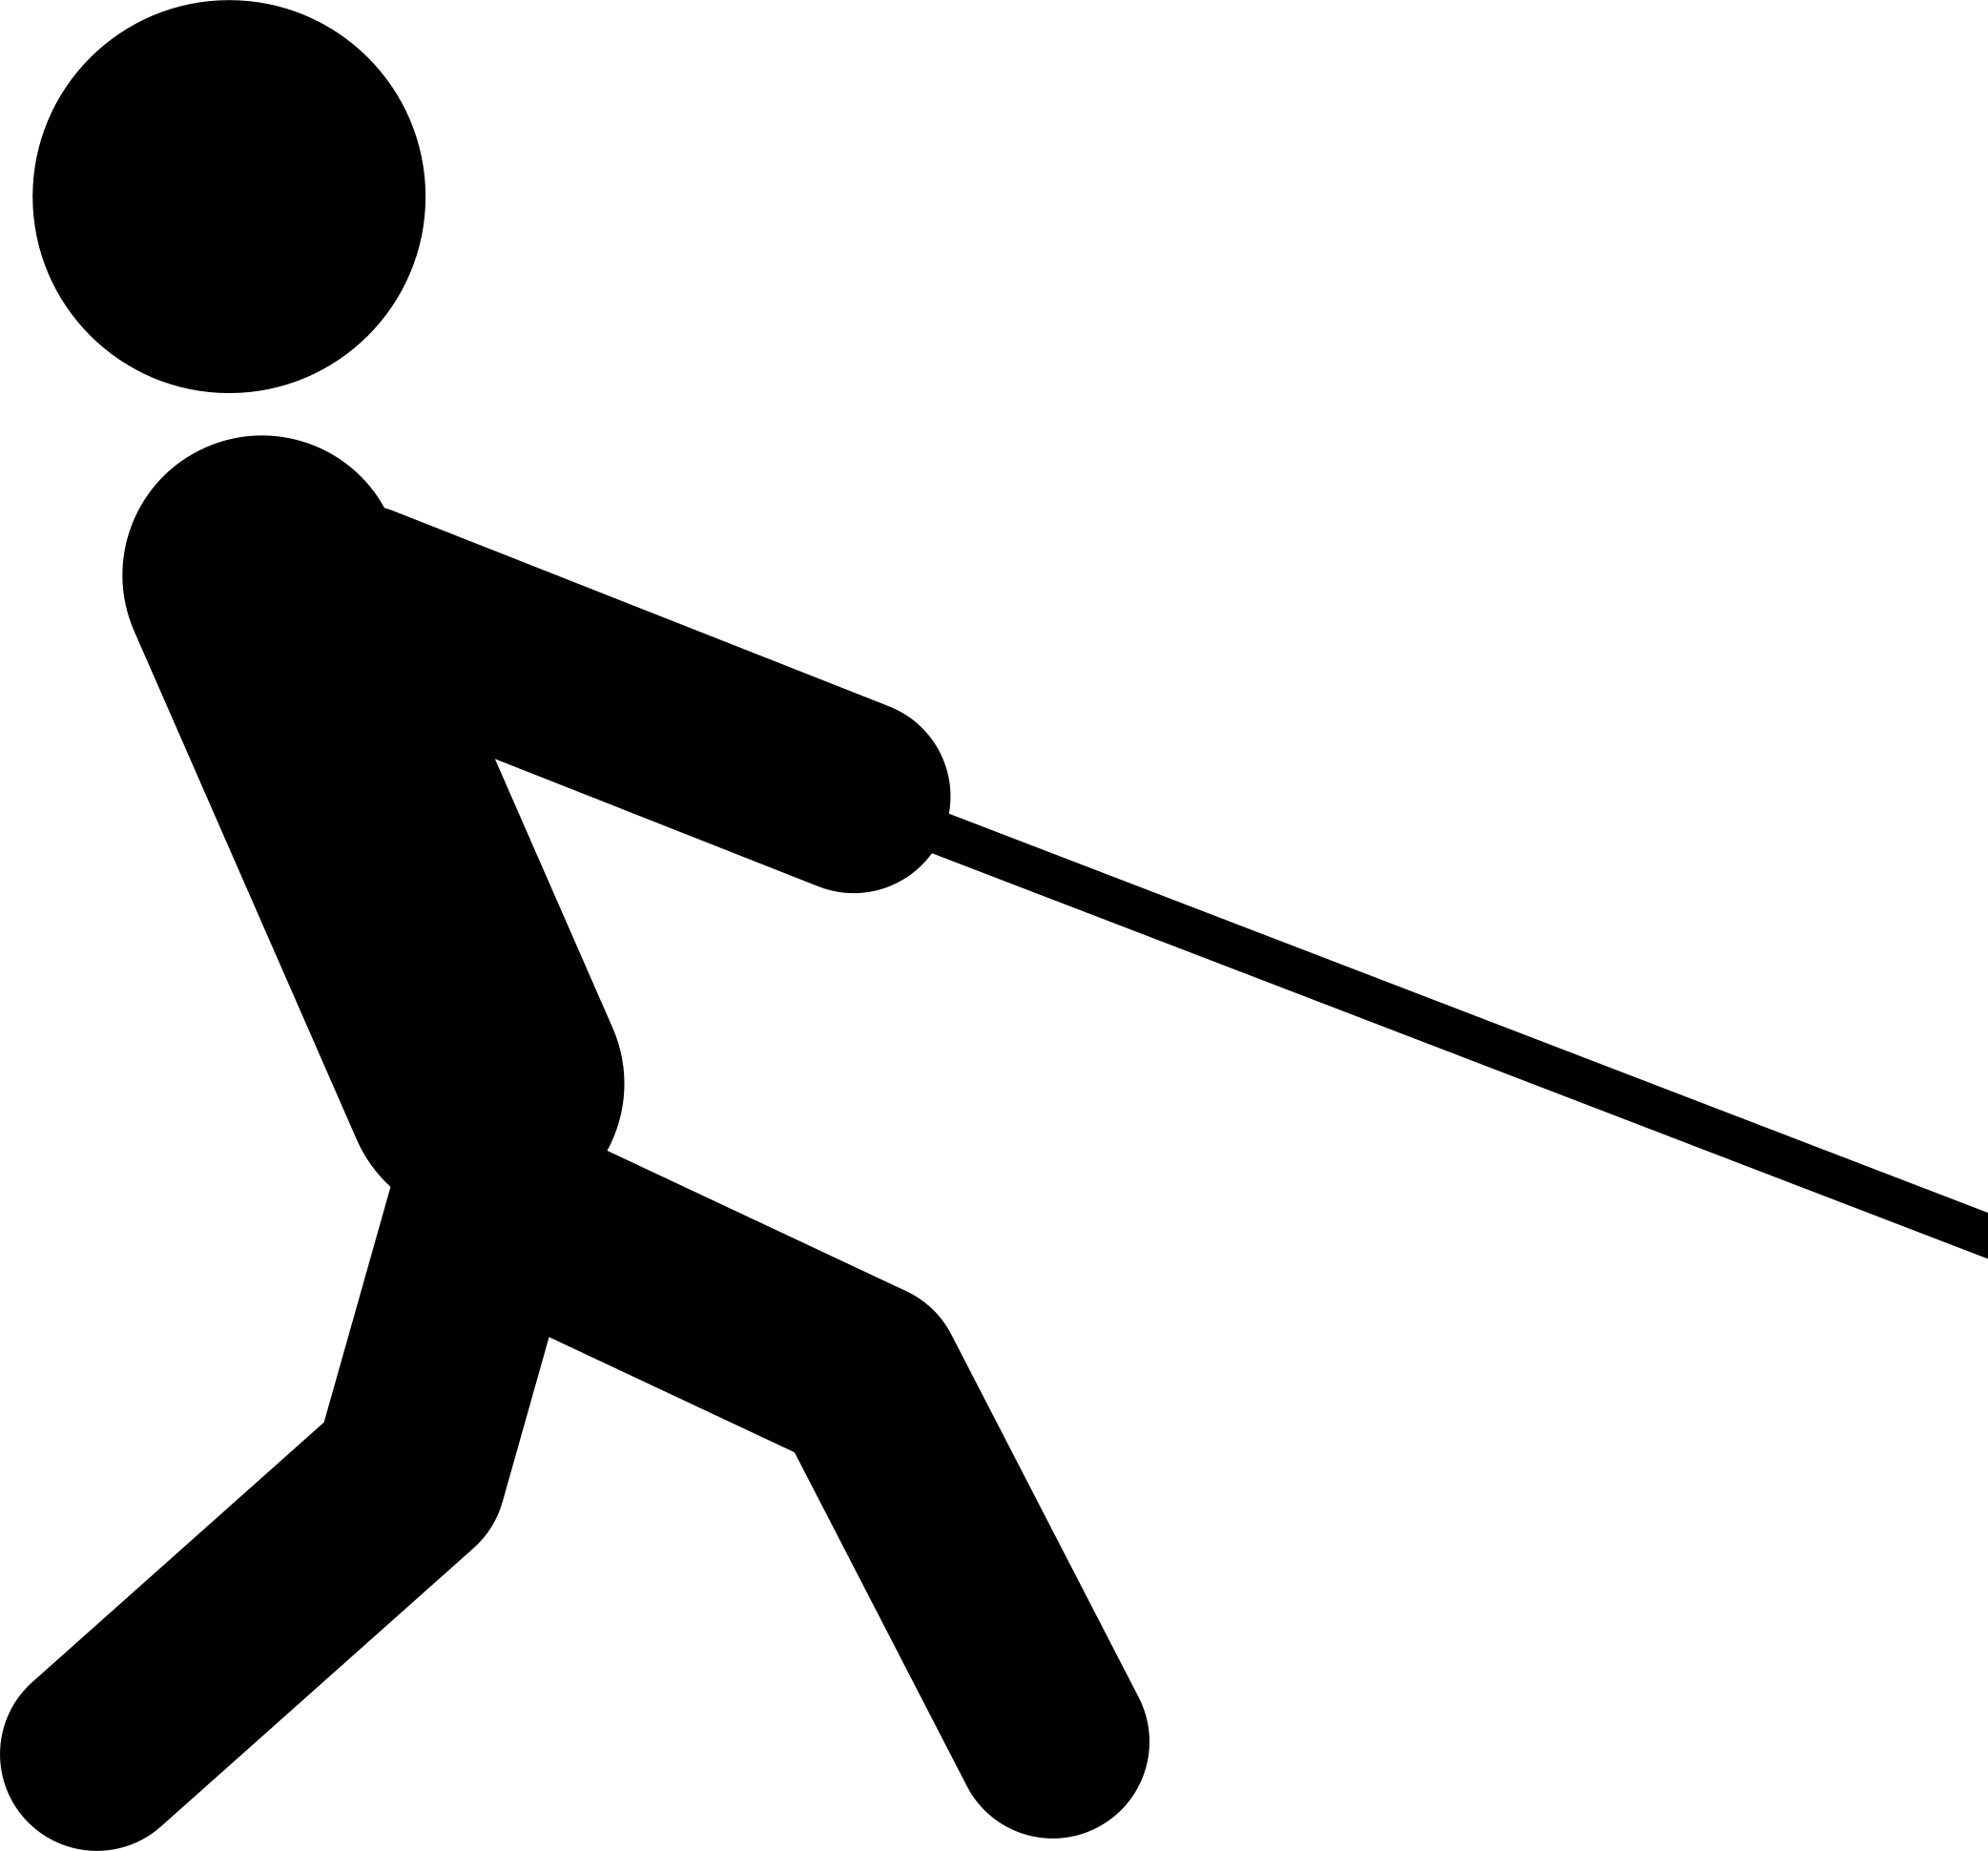
\includegraphics[height=3mm]{clipart/pull} \href{https://thenounproject.com/icon/pull-23535/}{pull} by \href{https://thenounproject.com/pavel.nikandrov/}{Pavel N} is licensed under \CCBYthree  ~(accessed 10 January 2023, modified)}

\begin{tikzpicture}
\draw(0,-0.005)node[left]{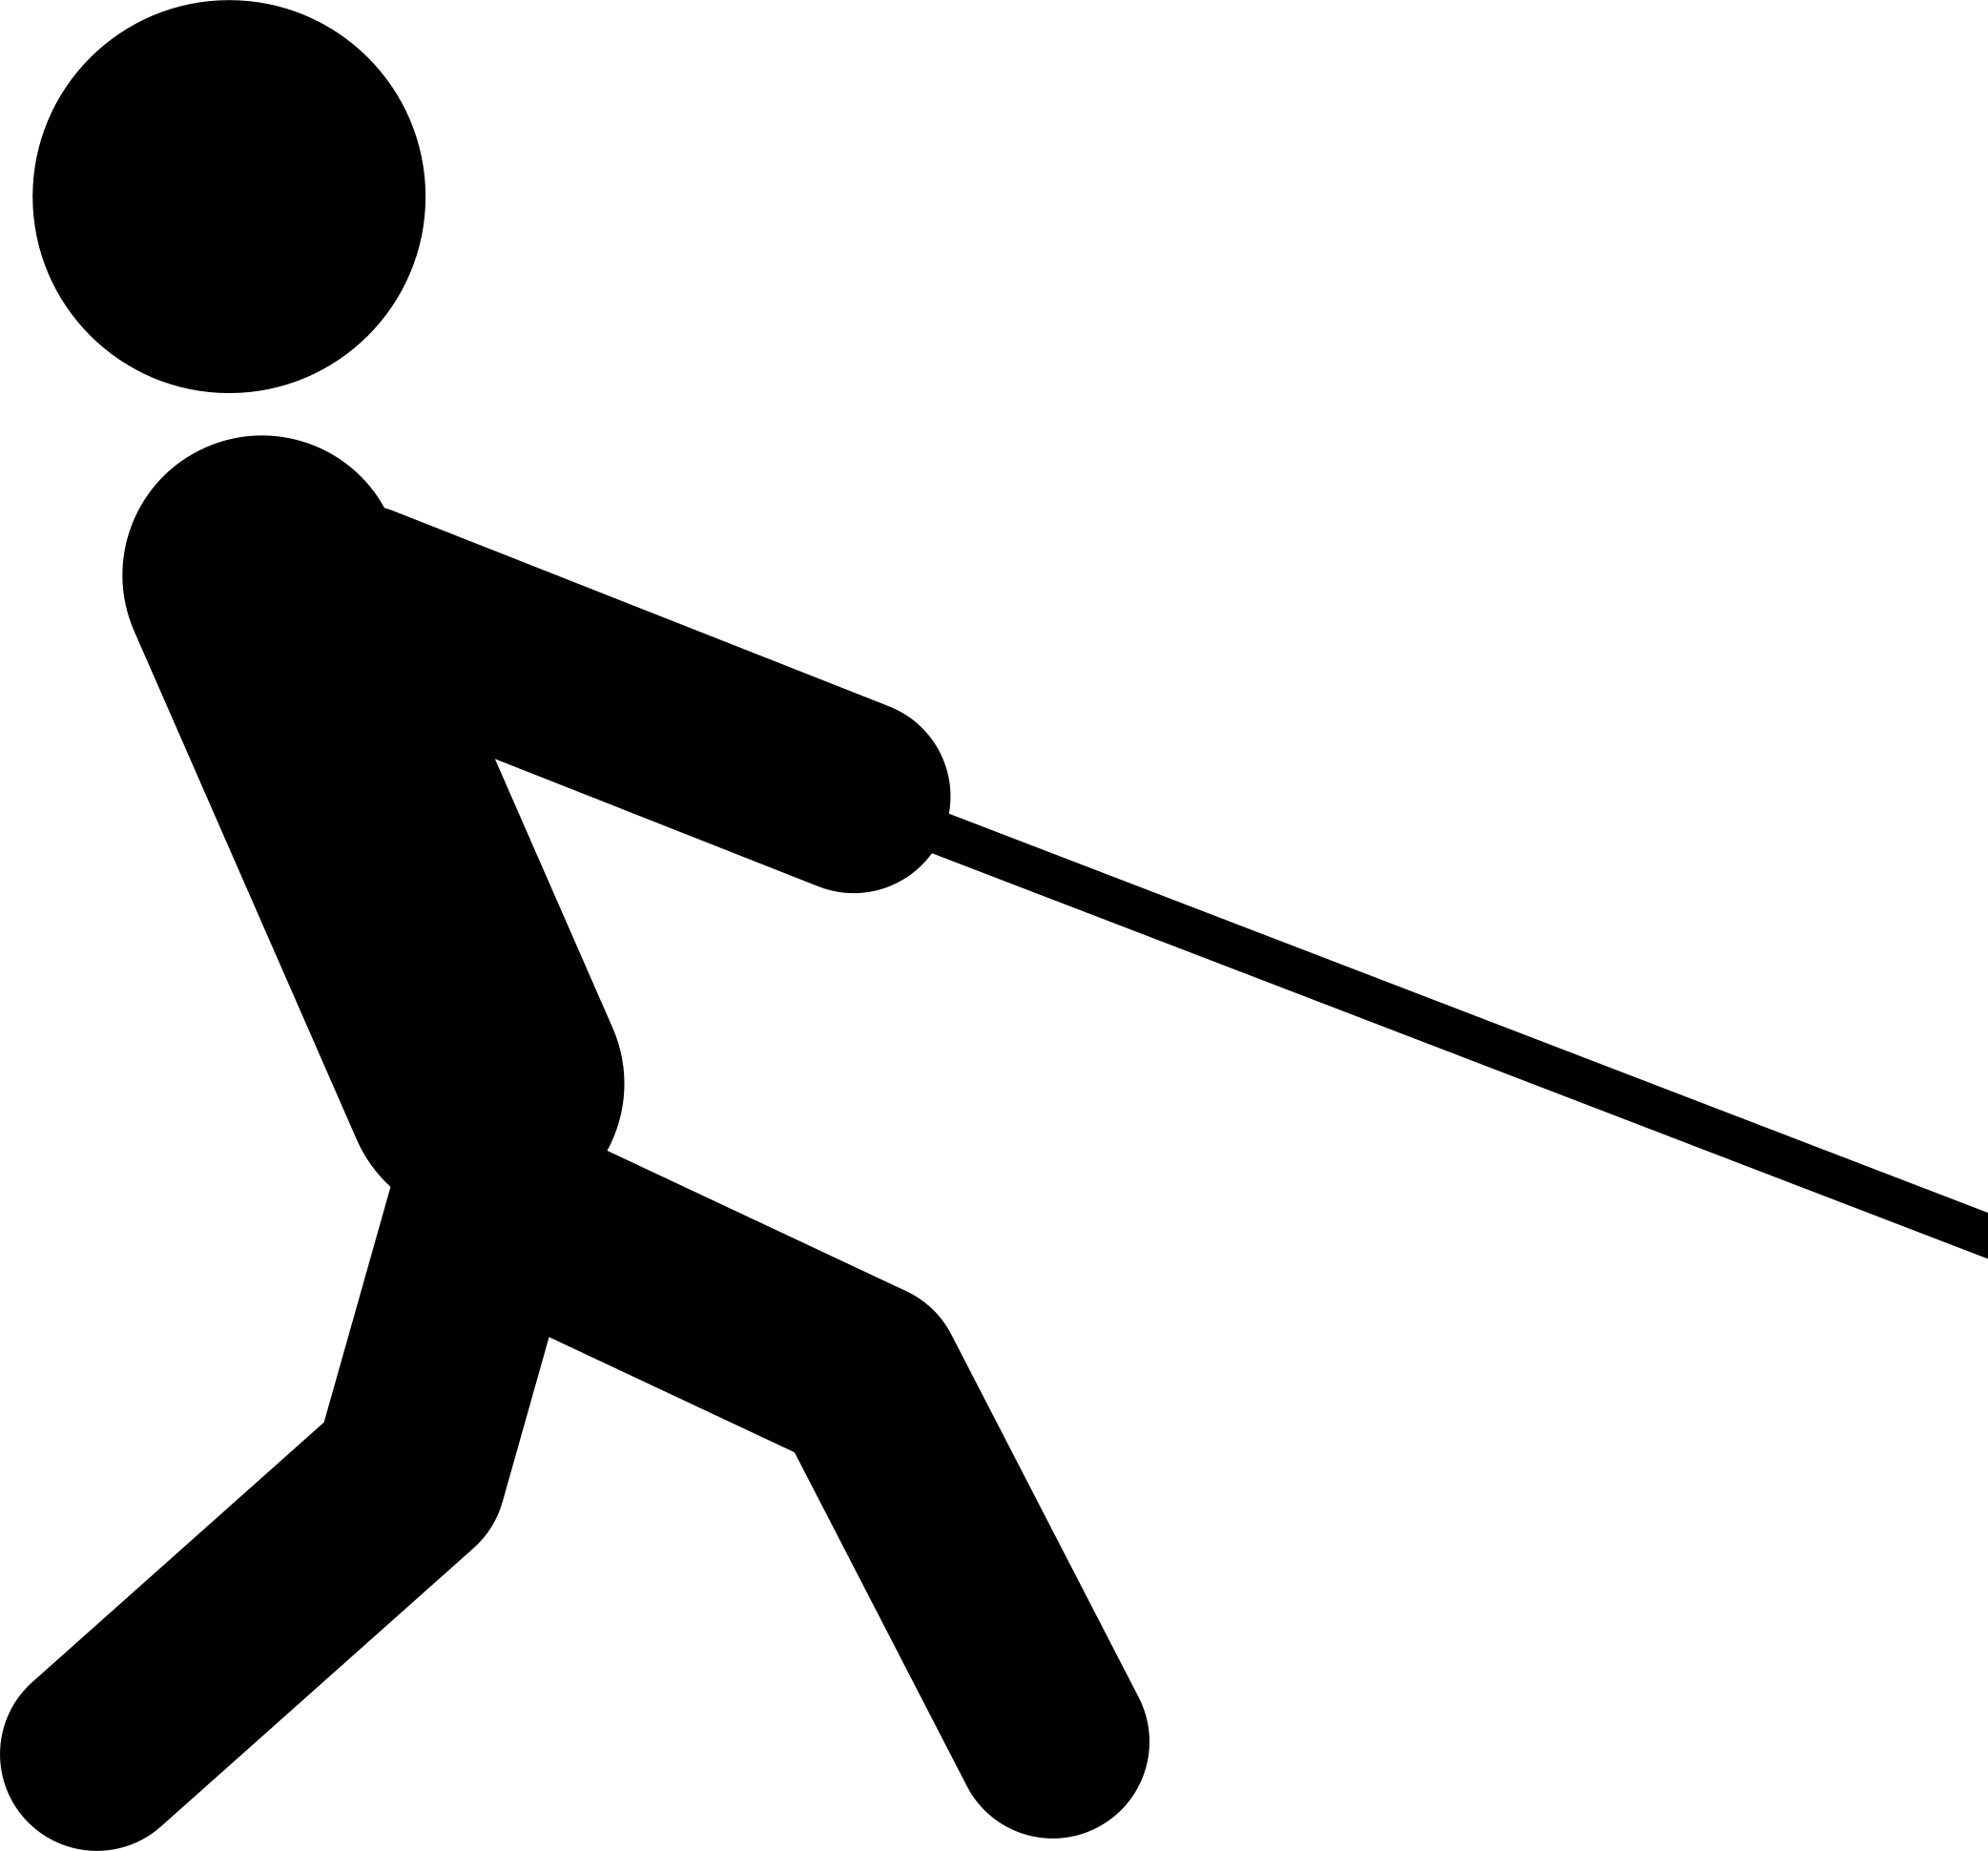
\includegraphics[width=1cm]{clipart/pull}};
\draw[line width=0.6pt] (-0.15,-.15)--(0.75,-.5)--+(0,-3);
\shadedraw[top color=white, bottom color=gray] (-2,-.5)--(.5,-.5)--(.5,-3.5) arc(180:360:2.5mm and 1mm)--(1,-.5)-|(1.5,-4)-|cycle;

\onslide<2|handout:0>{\draw[C3] (.75,-1)node[shape=circle,minimum size=2mm,inner sep=0,fill]{};}
\onslide<3|handout:0>{\draw[C3] (.75,-2.5)node[shape=circle,minimum size=2mm,inner sep=0,fill]{};}
\sonslide<5->{
	\draw[C3,line width=1mm] (.75,-1)--(.75,-1.3);
	\draw[|-|] (1.75,-0.5)--(1.75,-1.15)node[midway,right]{$y$};
	\draw[|-|] (.25,-1)--(.25,-1.3)node[midway,left]{$\dee y$};
	}
\end{tikzpicture}\hfill
\sonly<6->{\vspace{-1cm}
	\parbox{6cm}{
	The cable has density $\frac{5~\text{kg}}{10~\text{m}} = \frac12 \frac{\text{kg}}{\text{m}}$. A slice of length $\dee y$ has mass $\frac12 \dee y$ kg, so it is subject to a downward gravitational force of $\frac{g}{2} \dee y$ N, where $g$ is the acceleration due to gravity.
\\	
A slice $y$ metres below the top of the hole travels $y$ metres to get out of the hole, taking work $\frac{g}{2}y \ \dee y$. So the work required to life the entire cable out of the hole is:
\[\int_0^{10}\frac{g}{2}y \ \dee y = \left[\frac{g}{4}y^2\right]_0^{10}=25g~\text{J}\]
\vspace{2cm}
	}}
\pause
\only<-4>{\begin{itemize}[<+->]
\item A piece of the cable near the top of the hole isn't lifted very far.
\item A piece of the cable near the bottom of the hole is lifted farther.
\item Consider a small piece of cable starting $y$ metres from the top.
\end{itemize}}
\unote{Example~\eref{text}{eg:WKcable}}
\end{frame}

%----------------------------------------------------------------------------------------
\begin{frame}[t]
\StatusBar{1}{4}
\AnswerSpace
\only<4>{\MoreSpace}
\only<5>{\AnswerYes}
\begin{multicols}{2}\begin{tikzpicture}[yscale=0.8]
\shadedraw[bottom color=white, top color=M4, fill opacity=0.4](4,3) arc (0:360:2 cm and 5 mm);%container top
\onslide<4-|handout:0>{\shadedraw[top color=M3, bottom color=white] (4,1.2) arc(0:360:2cm and 5mm);} %slice top

%top molecule
\onslide<2|handout:0>{%high molecule
	\shadedraw[M3,ball color=M3](.6,2.5)arc(0:360:1mm);
	\draw[thick, M3,->] (.5,2.75)--(.5,3) to[bend right] (-.5,3);
	}
\onslide<3|handout:0>{%low molecule
	\shadedraw[M3,ball color=M3](.6,.5)arc(0:360:1mm);
	\draw[thick, M3,->] (.5,.75)--(.5,3) to[bend right] (-.5,3);
	}
%labels
\sonslide<6->{
	\draw[M3,|-|] (-.25,1)--(-.25,1.2)node[midway,left,xshift=-1mm]{$\dee y$};
	\draw[M3,|-|] (2,-.95)--(2,0.45)node[midway,left,xshift=-1mm]{$ y$};
	\draw[|-|] (2,3.25)--(4,3.25)node[midway,below]{$r$};
	\draw[|-|] (4.5,0)--(4.5,3)node[midway,right]{$h$};
	}

\shadedraw[left color=M4, right color=M4, middle color=white,fill opacity=0.4](0,3)--(0,0) arc (180:360:2cm and 1cm)--(4,3) arc (0:-180:2 cm and 5 mm);%container side
\onslide<4-|handout:0>{\shadedraw[left color=M3, right color=M3, middle color=white] (0,1) arc (180:360:2cm and 5mm)--(4,1.2) arc (0:-180:2cm and 5mm);}%slice side

\end{tikzpicture}
\columnbreak

\sonslide<6>{\hfill\parbox{.4\textwidth}{The volume of a cylindrical slice at height $y$ is $\pi r^2\, \dee y$. If the density of the liquid is $\rho$, then the mass of liquid in the slice is $\rho\cdot\pi r^2\, \dee y$. Let $g$ be the acceleration due to gravity. The force of gravity on the slice is $g\rho\cdot\pi r^2\, \dee y$.}}

\end{multicols}\vspace{-1mm}
\only<-3|handout:1>{
A cylinder is filled with a liquid that we will pump out the top.
\begin{itemize}
\item<2-> To pump out a molecule from the top of the container, we don't have to work against gravity for very far.
\item<3-> To pump out a molecule from the bottom of the container, we have to work against gravity for a longer distance.
\end{itemize}}
\only<4|handout:2>{\begin{itemize}[<+->]
\item Every molecule at the same height has the same distance to travel to reach the top of the container. So, we'll chop up the tank into thin horizontal slices.
\end{itemize}}

\sonly<6>{

	 Liquid in the slice needs to travel to the top of the container, a distance of $h-y$. So the work required to pump out a single slice at height $y$ is $(h-y)g\rho\cdot\pi r^2\, \dee y$. All together, the work to empty the container is
	 \[\int_0^h(h-y)g\rho\cdot\pi r^2\, \dee y.\]
	}
\sonly<7>{\begin{align*}
\int_0^h (h-y)g\rho \cdot \pi r^2\,\dee y & = g\rho\cdot \pi r^2\int_0^h(h-y)\,\dee y\\
&=g\rho\cdot \pi r^2\left[hy-\tfrac12y^2\right]_0^h\\
&=g\rho\cdot \pi r^2\cdot \tfrac{h^2}{2}
\end{align*}}
\unote{Example~\eref{text}{eg:WKdrum}}
\end{frame}
%----------------------------------------------------------------------------------------

%----------------------------------------------------------------------------------------
\begin{frame}[t]
\AnswerYes<5>
\sNoSpace<5>
\nsNoSpace<6>
\StatusBar{1}{6}
\begin{block}{Hooke's Law}
When a (linear) spring is stretched (or
compressed) by $x$ units beyond its natural length, it exerts a force of
magnitude $kx$, where the constant $k$ is the spring constant of that spring.
\end{block}

\begin{center}
\begin{tikzpicture}
\draw[ultra thick] (0,1)|-(3.5,0);
\xcoord{2}{}
\foreach \x[count=\N] in {2,2.25,...,3.25}{
	\ifnum \N=2
		\newcommand{\handoutslide}{1}
		\else
		\newcommand{\handoutslide}{0}
	\fi
\onslide<+|handout:\handoutslide>{
	\xcoord{\x}{}
	\DIVIDE{\x}{14.9}{\sl}
	\SUBTRACT{\sl}{0}{\SL}
	\draw [decorate,decoration={coil,aspect=0.3,segment length=\SL cm,amplitude=3mm}] (0,0.5)--(\x,0.5);
	\draw(\x,.5)--(\x+.5,.5);
	\ifdim \x pt > 2 pt
		\draw[decorate, decoration={brace,amplitude=6pt,mirror}] (2,-.3)--(\x,-.3)node[midway,below,yshift=-3mm]{$x$};
		
		\draw (\x+.4,.75)node[right]{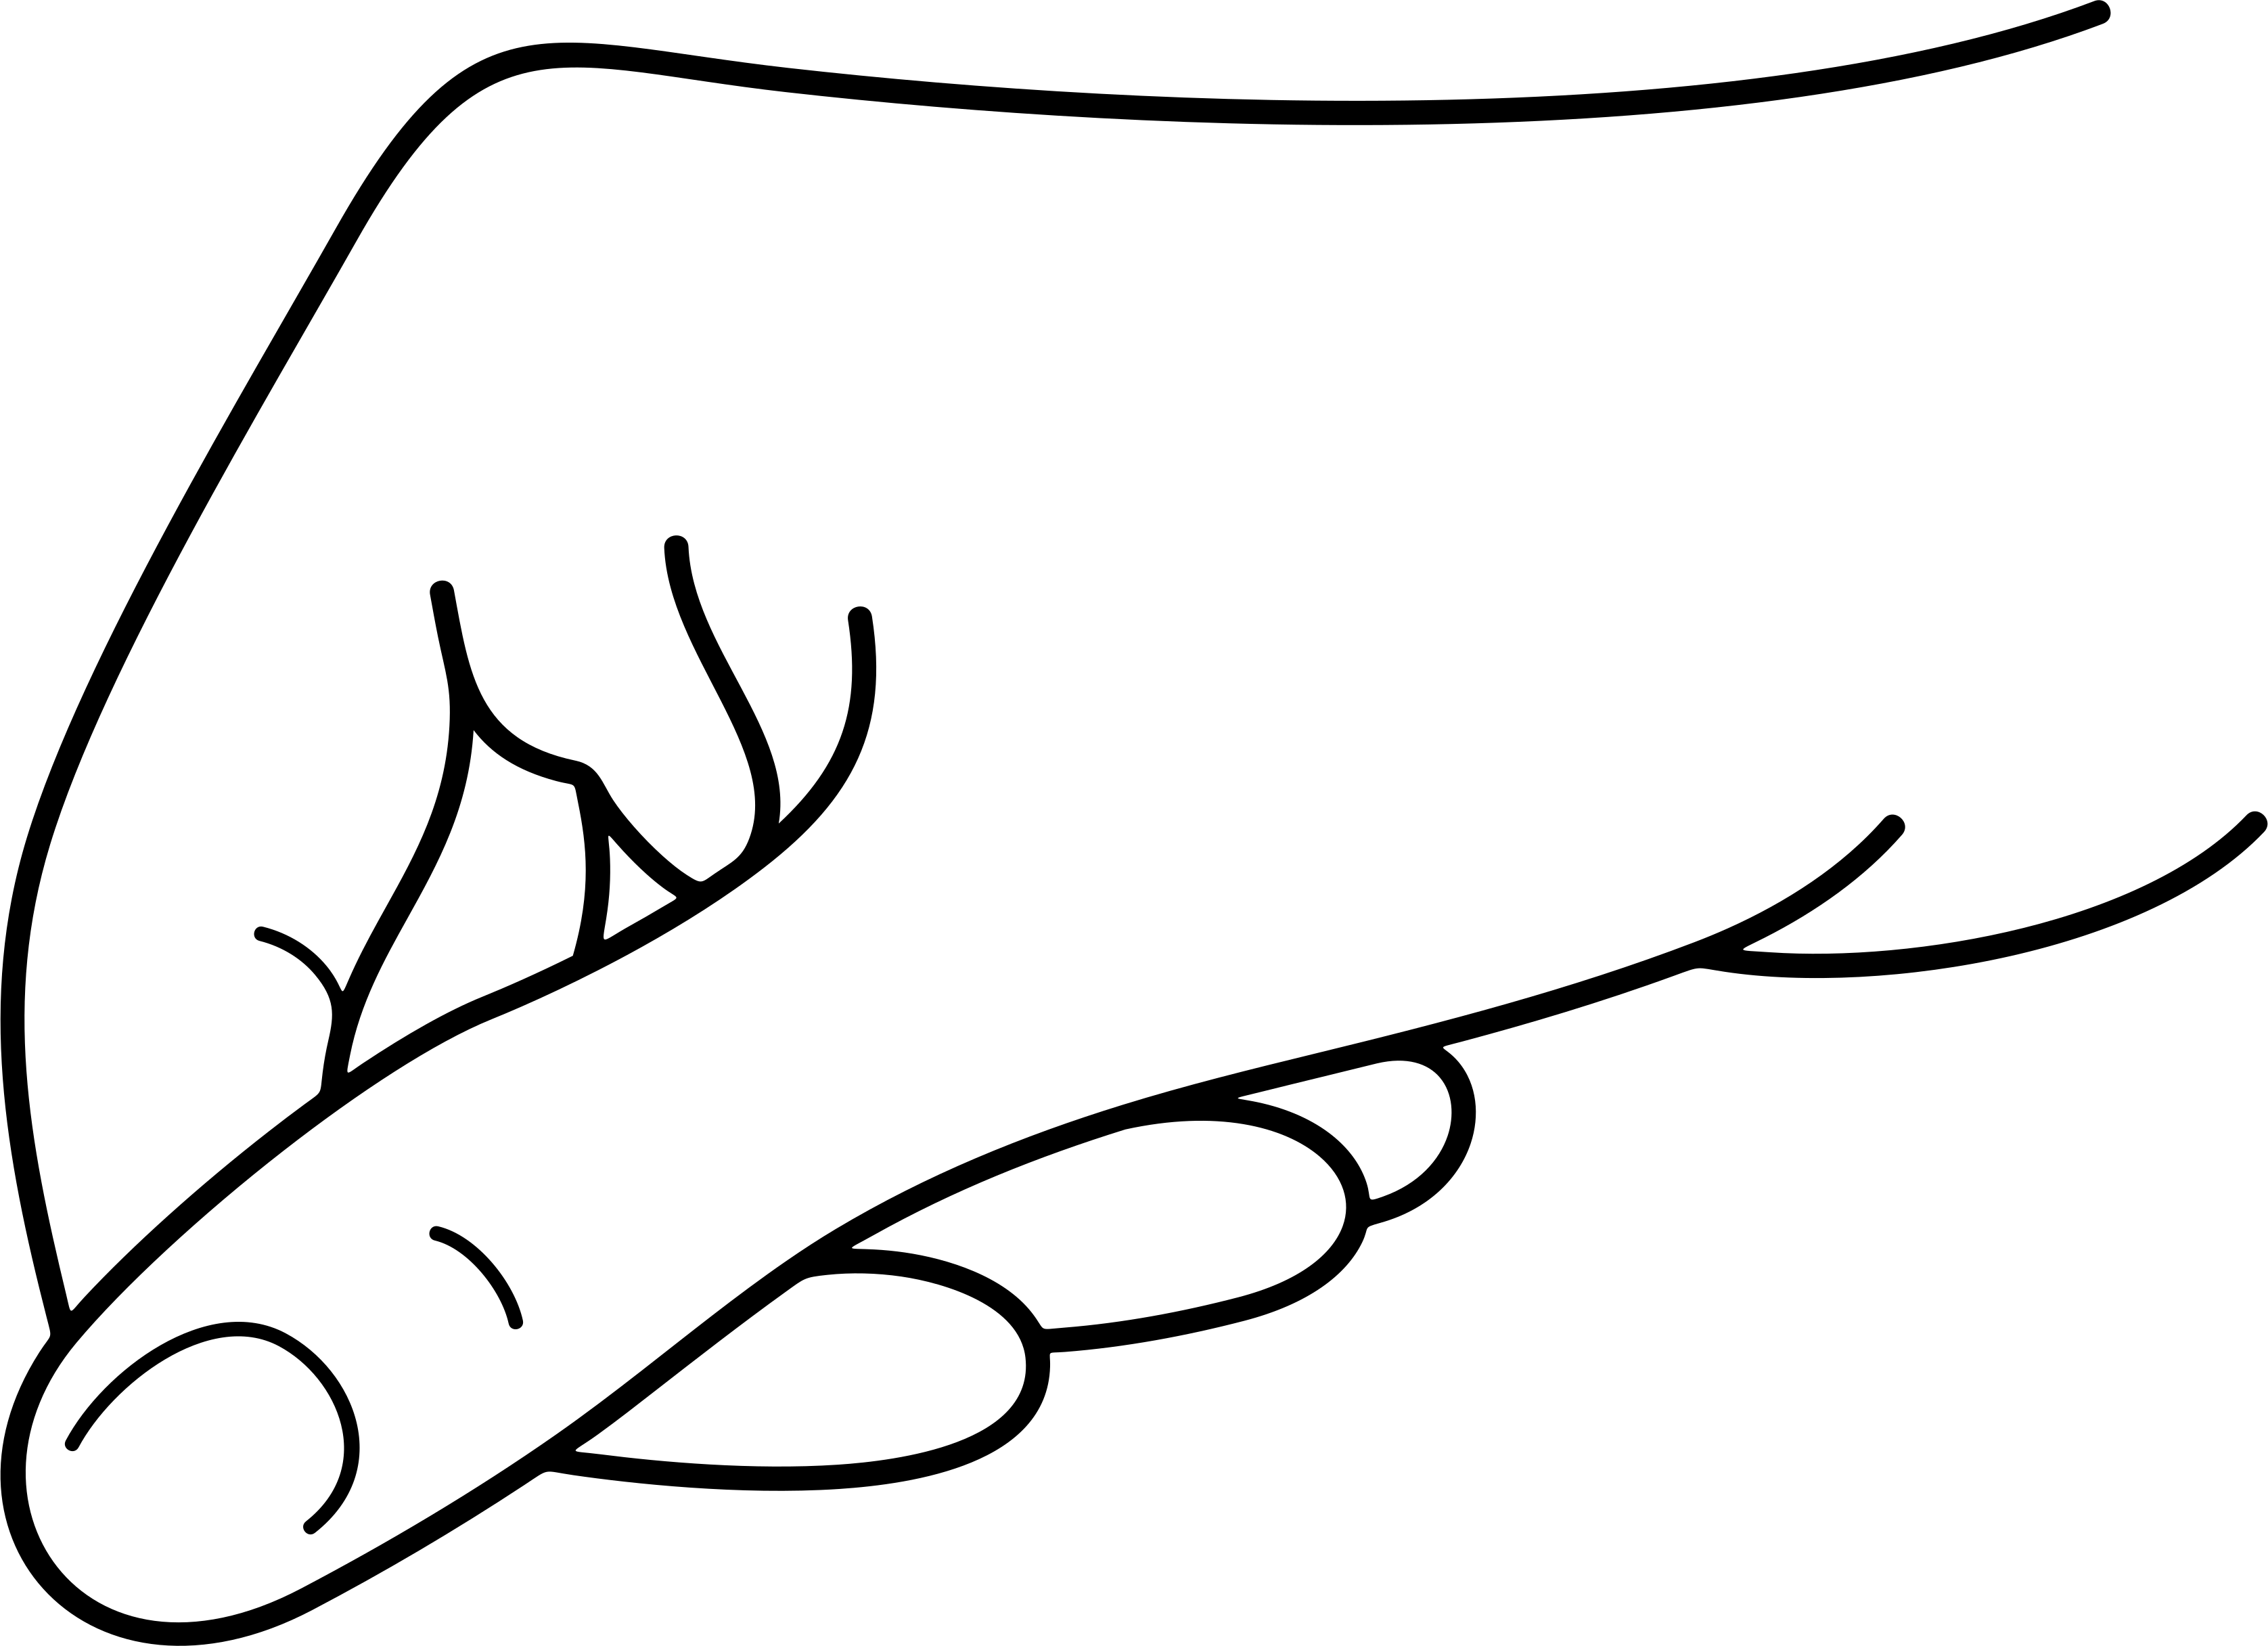
\includegraphics[width=1cm]{clipart/grab}};
		\index{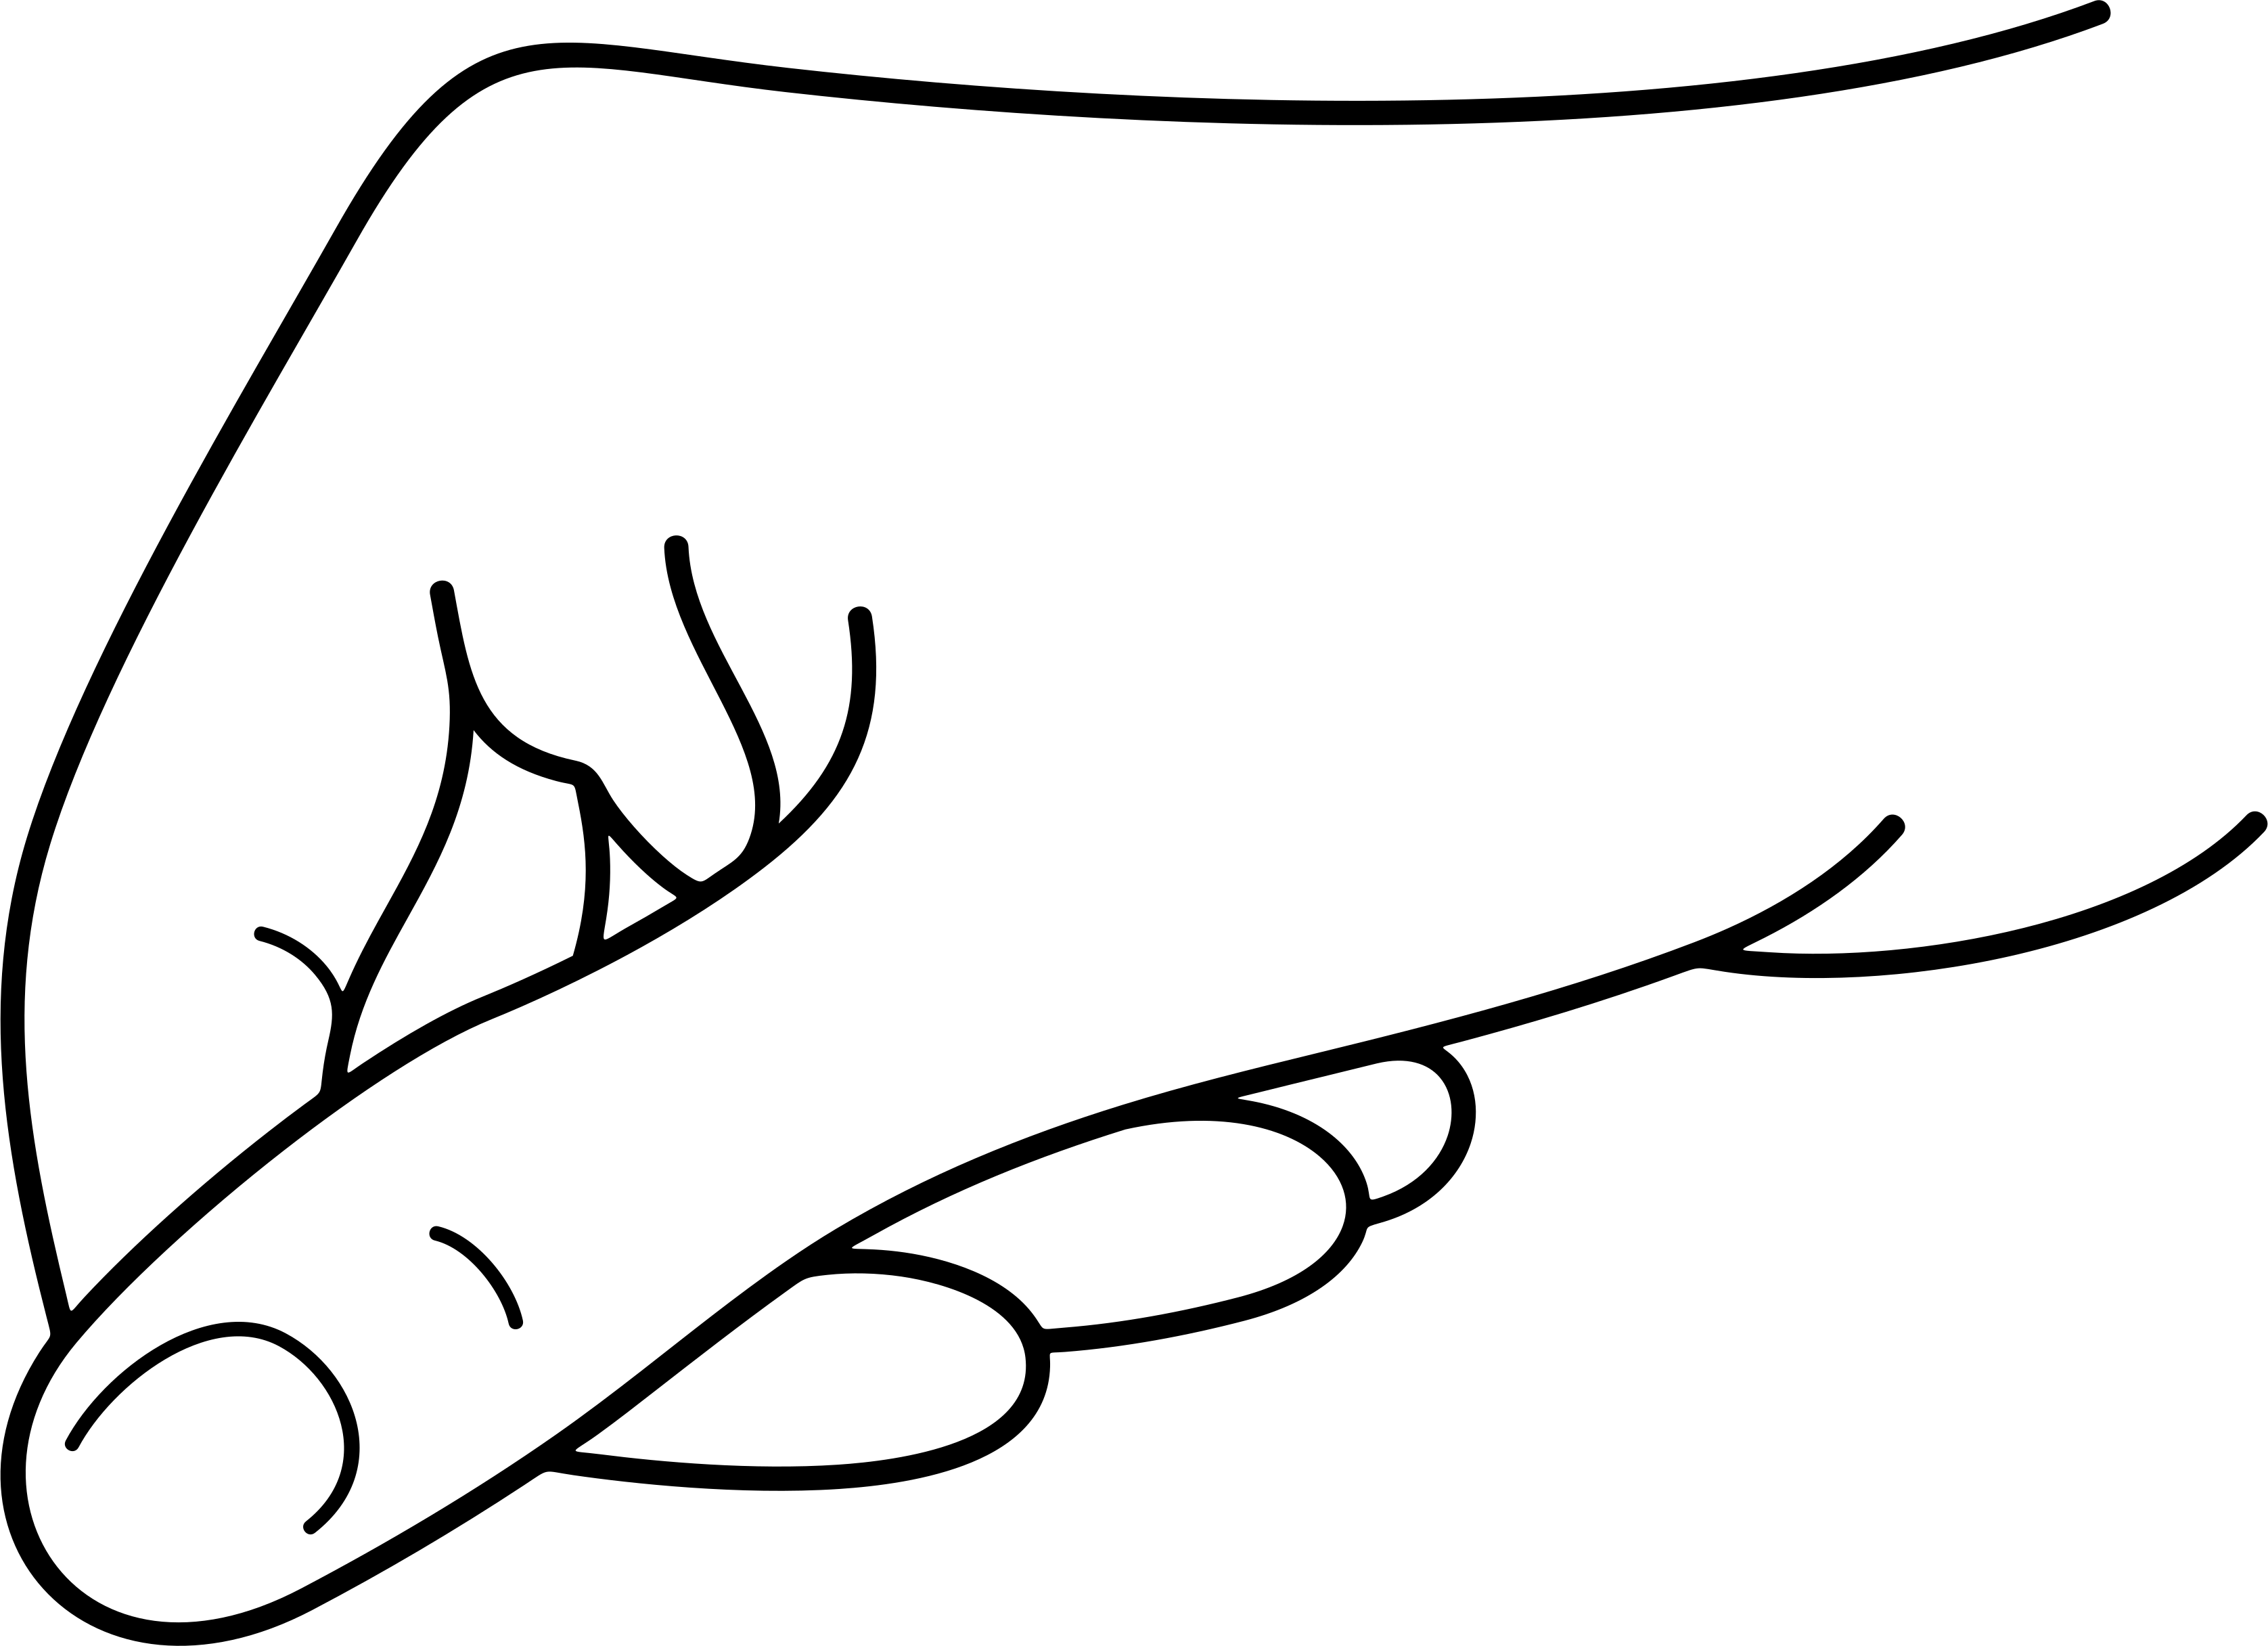
\includegraphics[height=3mm]{clipart/grab} \href{https://thenounproject.com/icon/hand-grab-2228970/}{HAND GRAB} by \href{https://thenounproject.com/a.panasovsky/}{Oleksandr Panasovskyi} is licensed under \CCBYthree ~(accessed 10 January 2023)}
	\fi}
}

\end{tikzpicture}\end{center}

\onslide<2->{Suppose we want to stretch a string from $a$ units beyond its natural length to $b$ units beyond its natural length. The force of the spring at position $x$ is $kx$, for some constant $k$. So, the work required is:
}

\sonslide<6->{ \[\int_a^b kx \ \dee x = \frac{k}{2}\left(b^2-a^2\right)\]}
\unote{Example~\eref{text}{eg:WKhookes}}
\end{frame}
%----------------------------------------------------------------------------------------
%----------------------------------------------------------------------------------------

\begin{frame}[t]
\AnswerYes<2,4>
\sMoreSpace<3>
\nsStatusBar{1}{3}
\only<1|handout:0>{\index{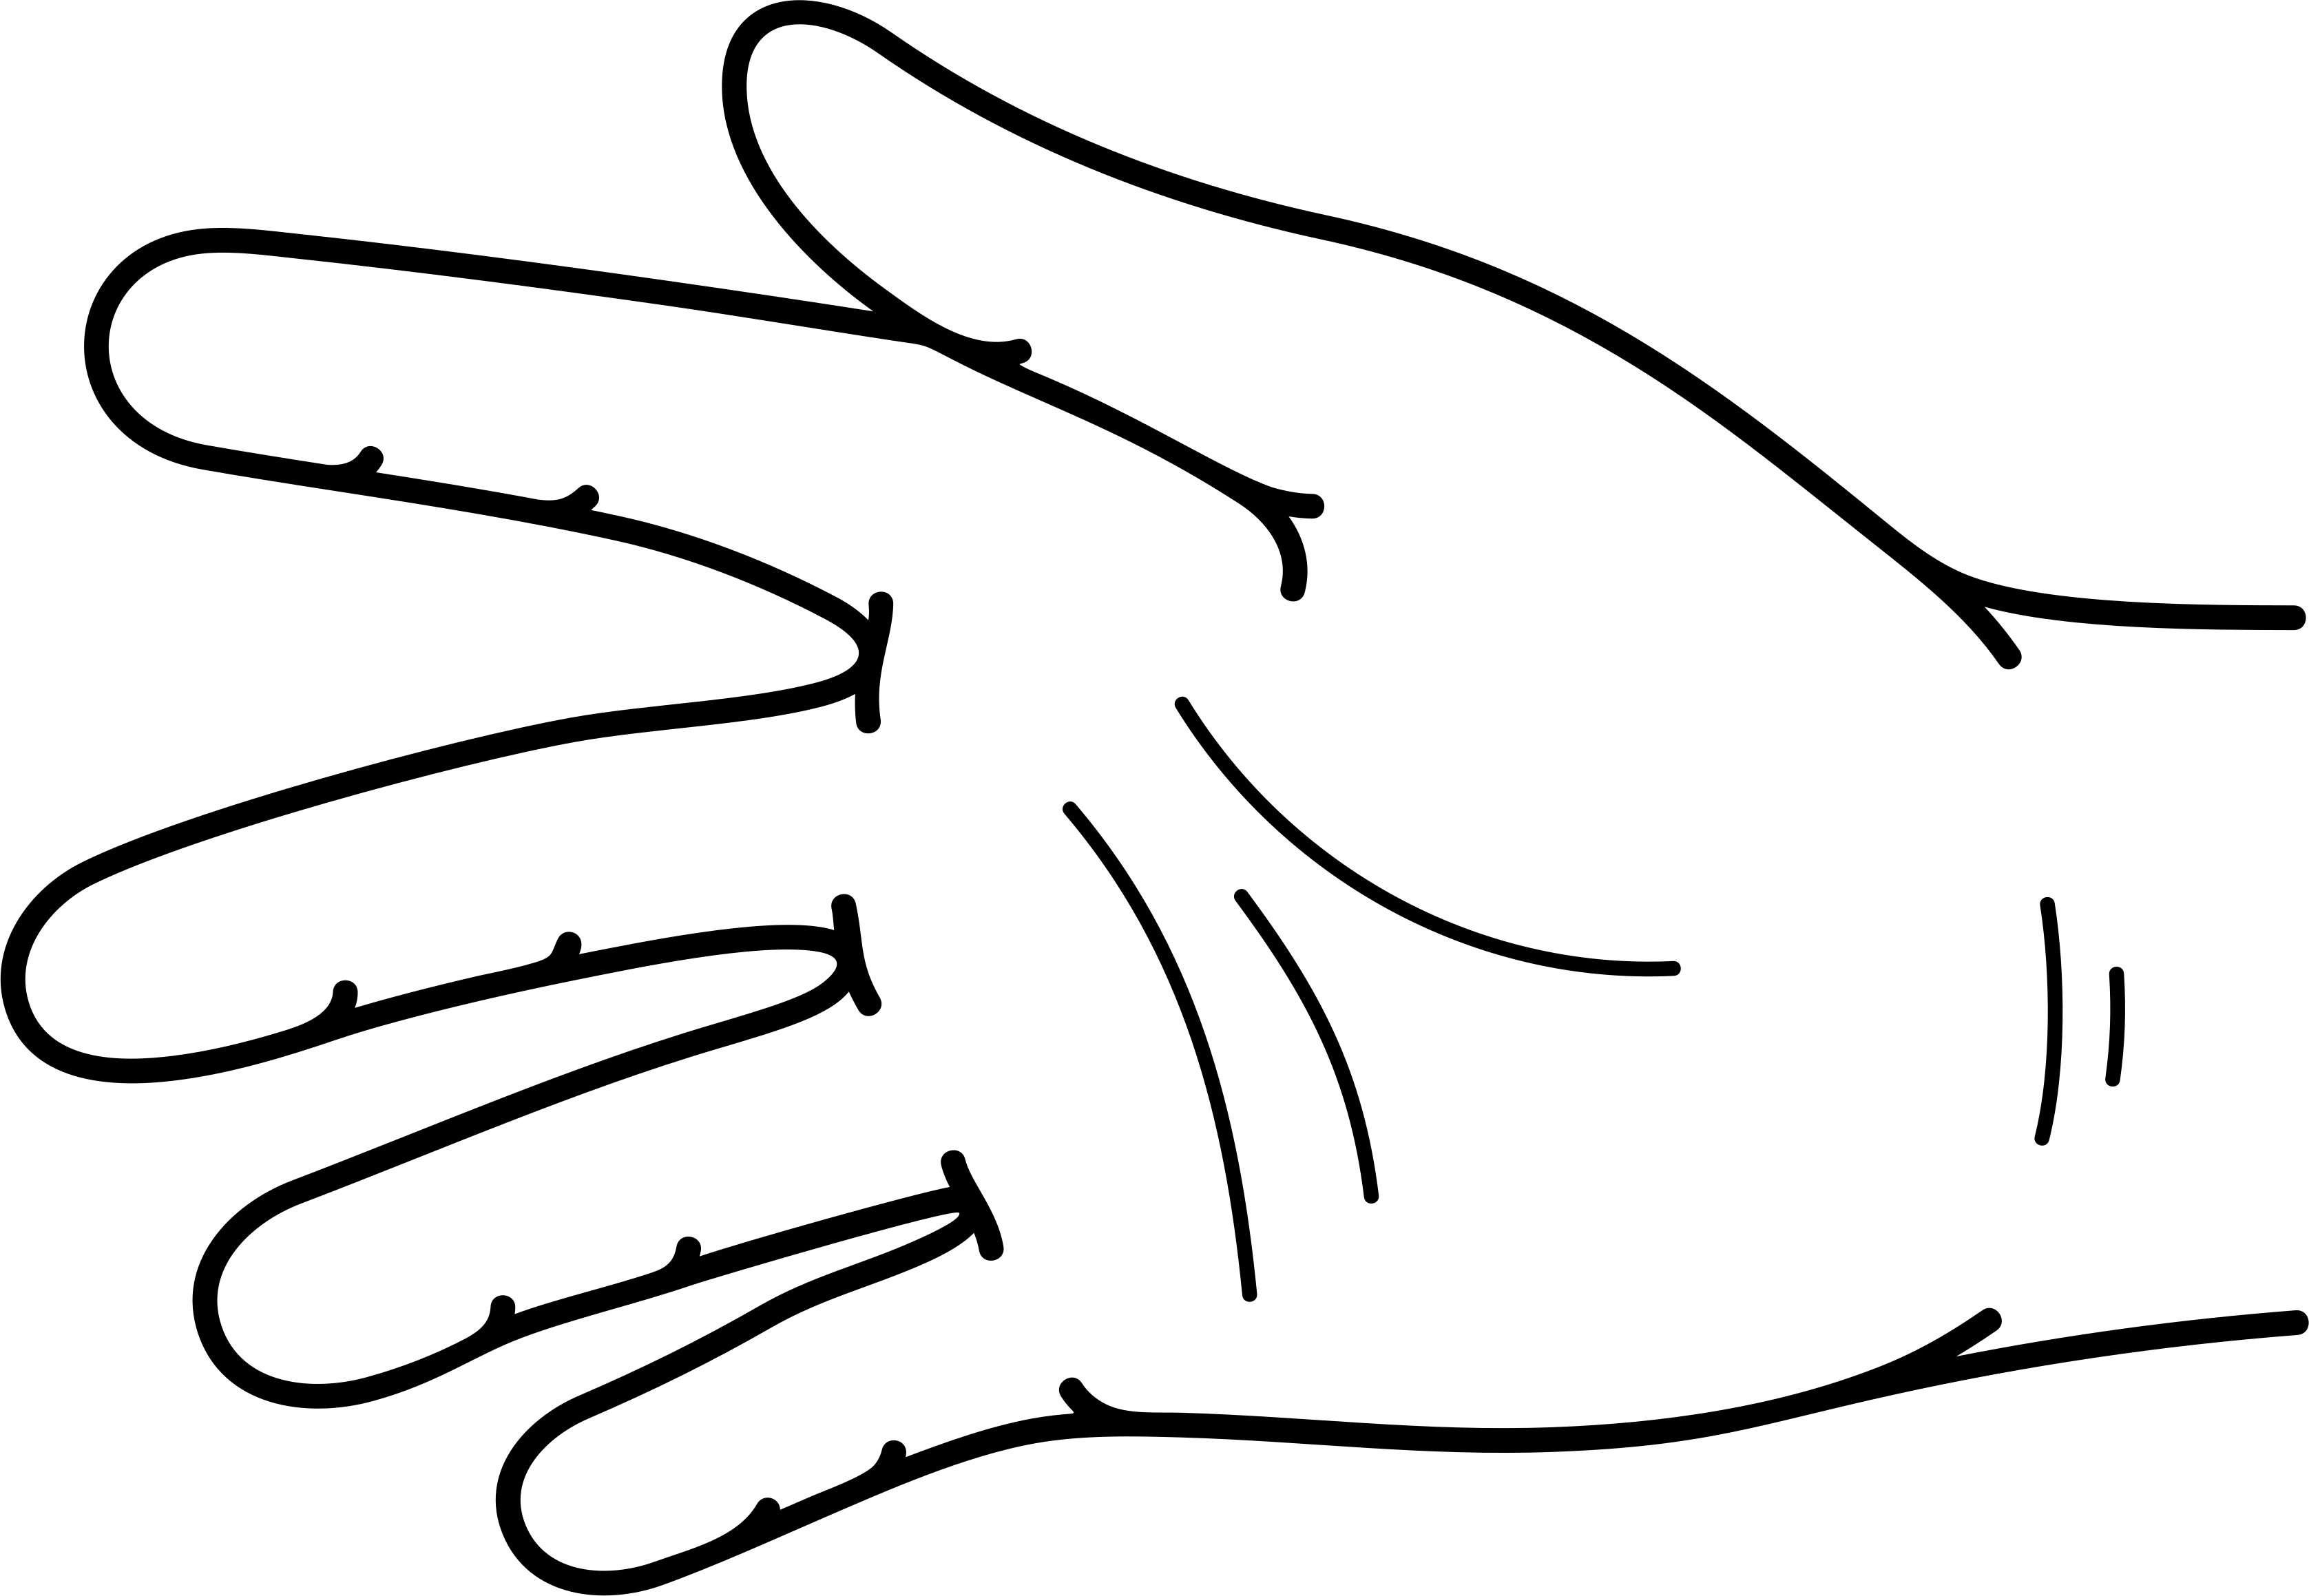
\includegraphics[height=3mm]{clipart/nograb} \href{https://thenounproject.com/icon/grabbing-hand-2335578/}{Grabbing Hand} by \href{https://thenounproject.com/a.panasovsky/}{Oleksandr Panasovskyi} is licensed under \CCBYthree ~(accessed 10 January 2023)}}
\only<2->{\index{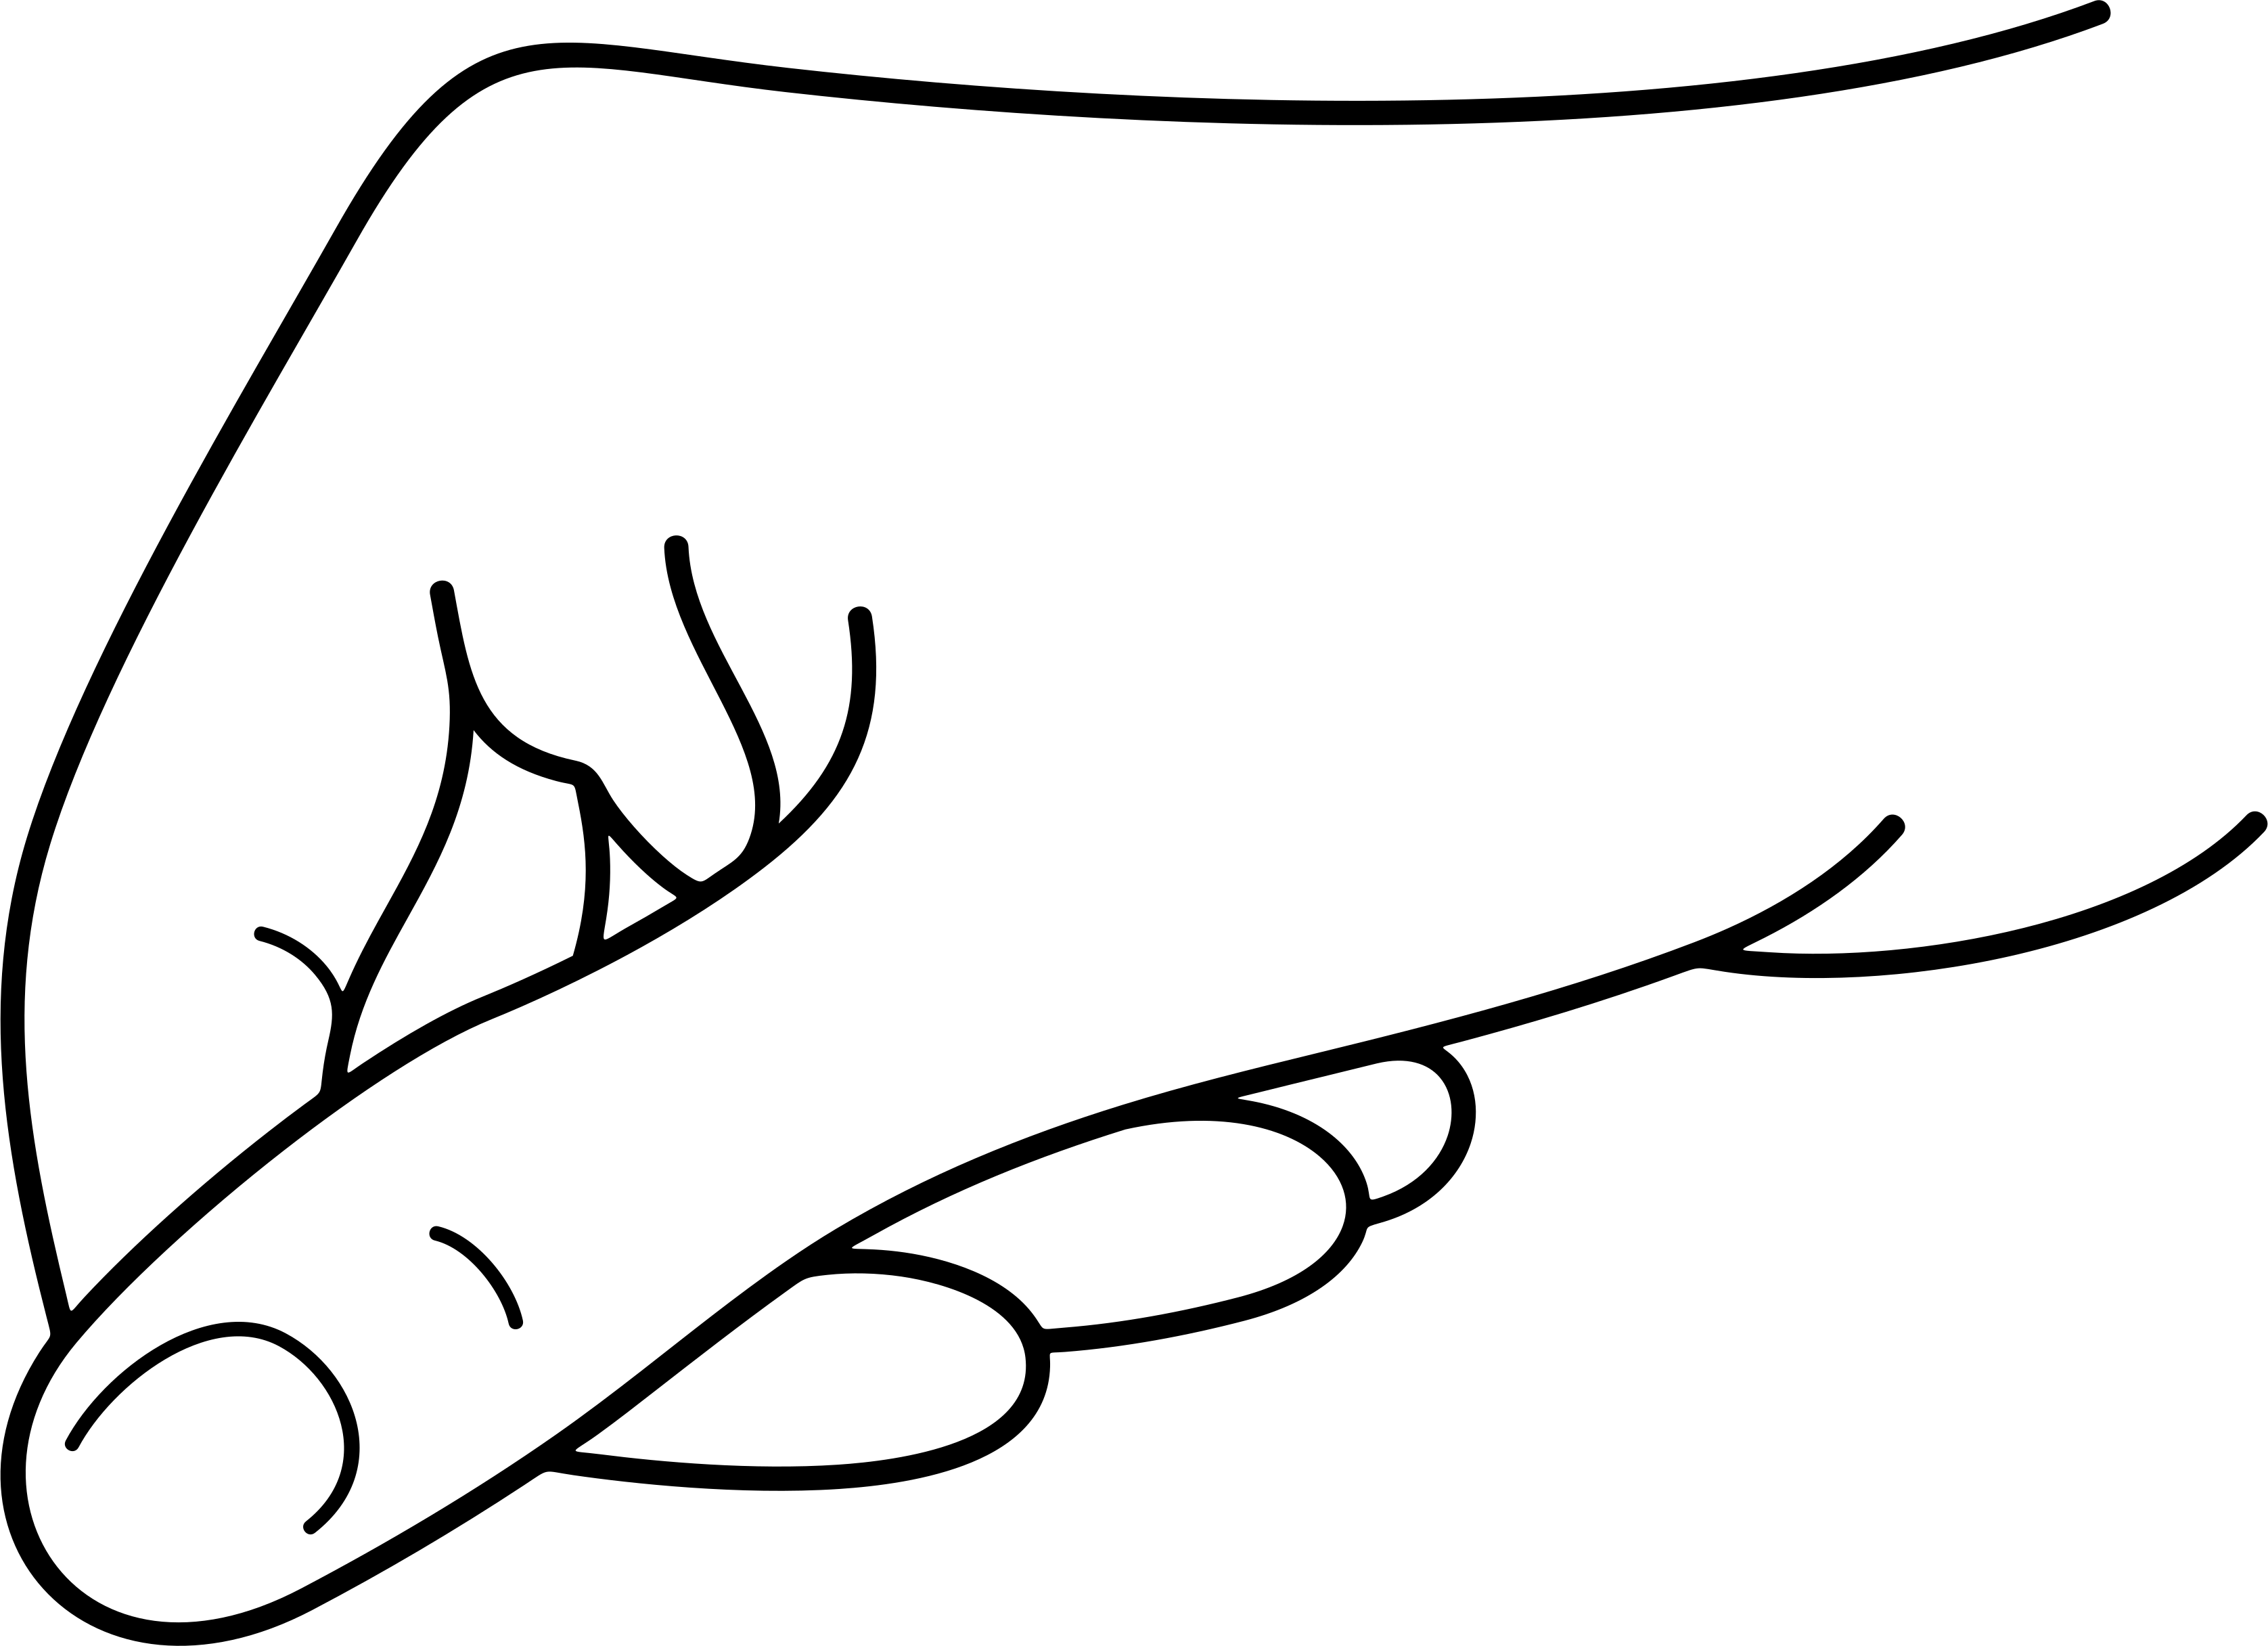
\includegraphics[height=3mm]{clipart/grab} \href{https://thenounproject.com/icon/hand-grab-2228970/}{HAND GRAB} by \href{https://thenounproject.com/a.panasovsky/}{Oleksandr Panasovskyi} is licensed under \CCBYthree ~(accessed 10 January 2023)}}

A spring has a natural length of $0.1$ m. If a $12$ N force is
needed to keep it stretched to a length of $0.12$ m, how much work
is required to stretch it from $0.12$ m to $0.15$ m?

\begin{center}
\begin{tikzpicture}
\draw[ultra thick] (0,1)|-(6.5,0);
\xcoord{4}{0.1}
\onslide<1|handout:0>{
	\draw [decorate,decoration={coil,aspect=0.3,segment length=.2 cm,amplitude=3mm}] (0,0.5)--(4.1,0.5);
	\draw(4.1,.5)--+(.5,0);
	\draw (4.75,.5)node[right]{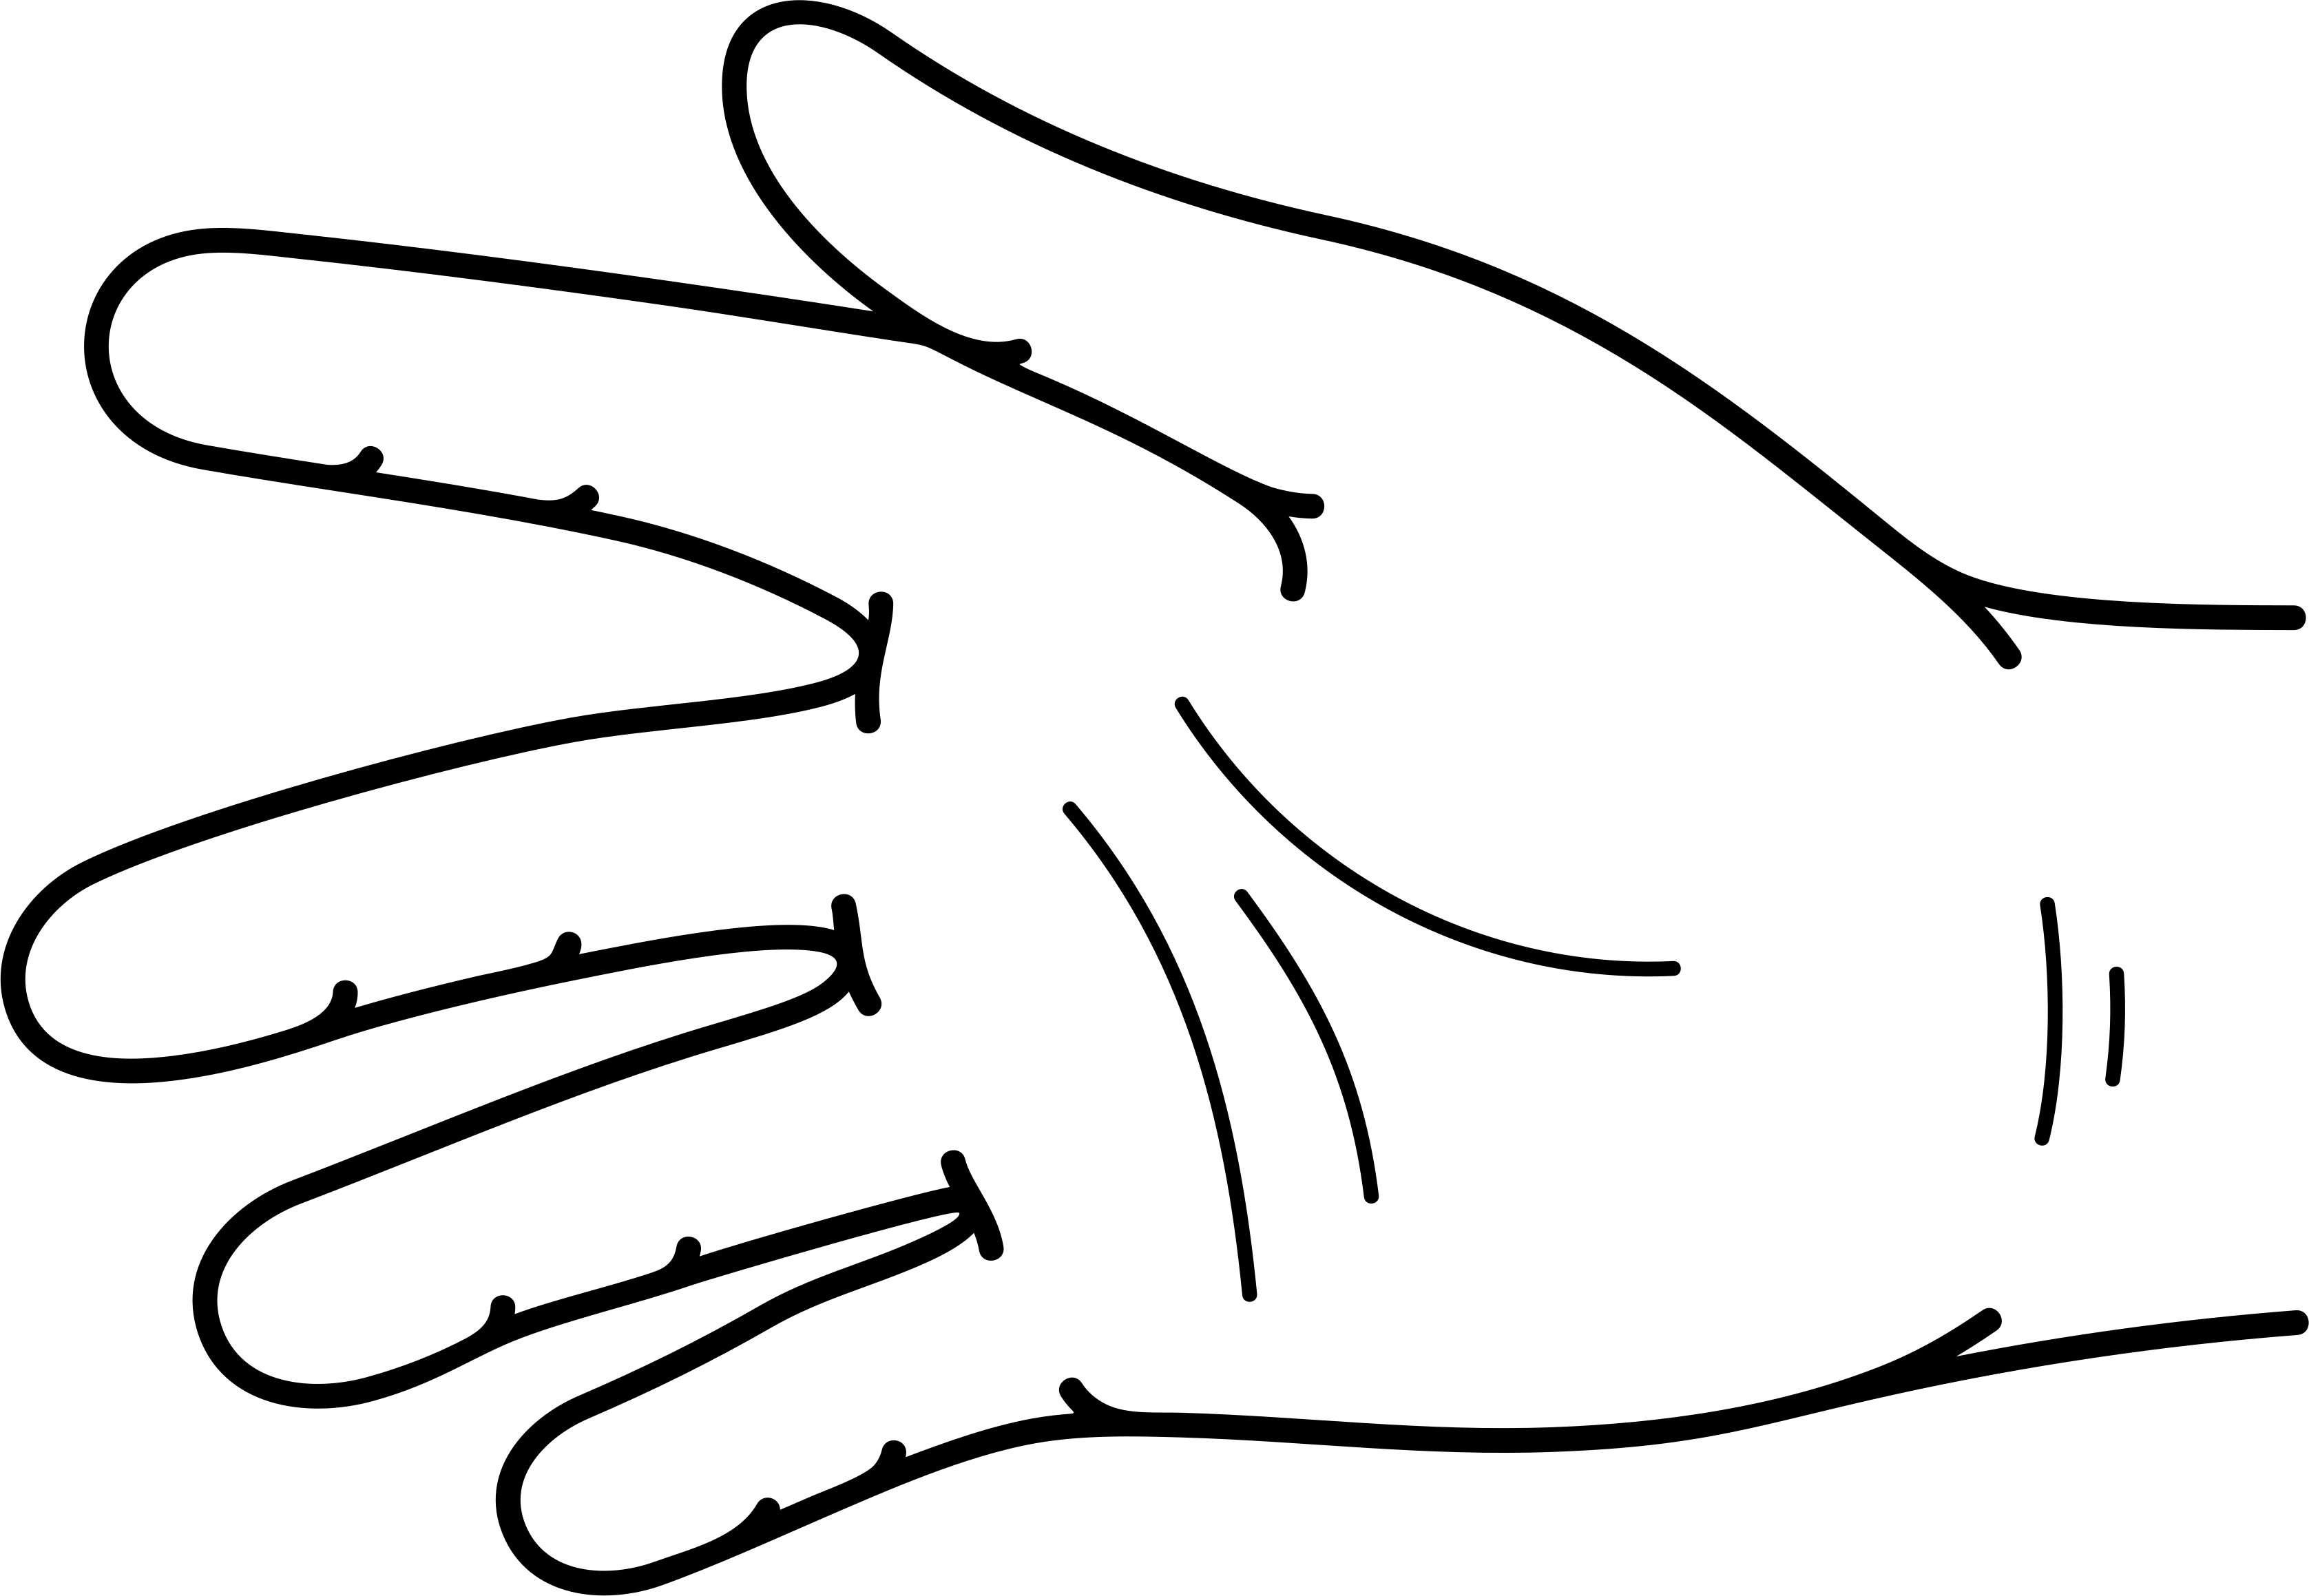
\includegraphics[width=1cm]{clipart/nograb}};
	}

\onslide<2->{\xcoord{4.8}{0.12}}
\snshonslide{2-3}{2}{0}{
	\draw [decorate,decoration={coil,aspect=0.3,segment length=.24 cm,amplitude=3mm}] (0,0.5)--(4.9,0.5);
	\draw (4.9,0.5)--+(.5,0);
	\draw (5.25,.75)node[right]{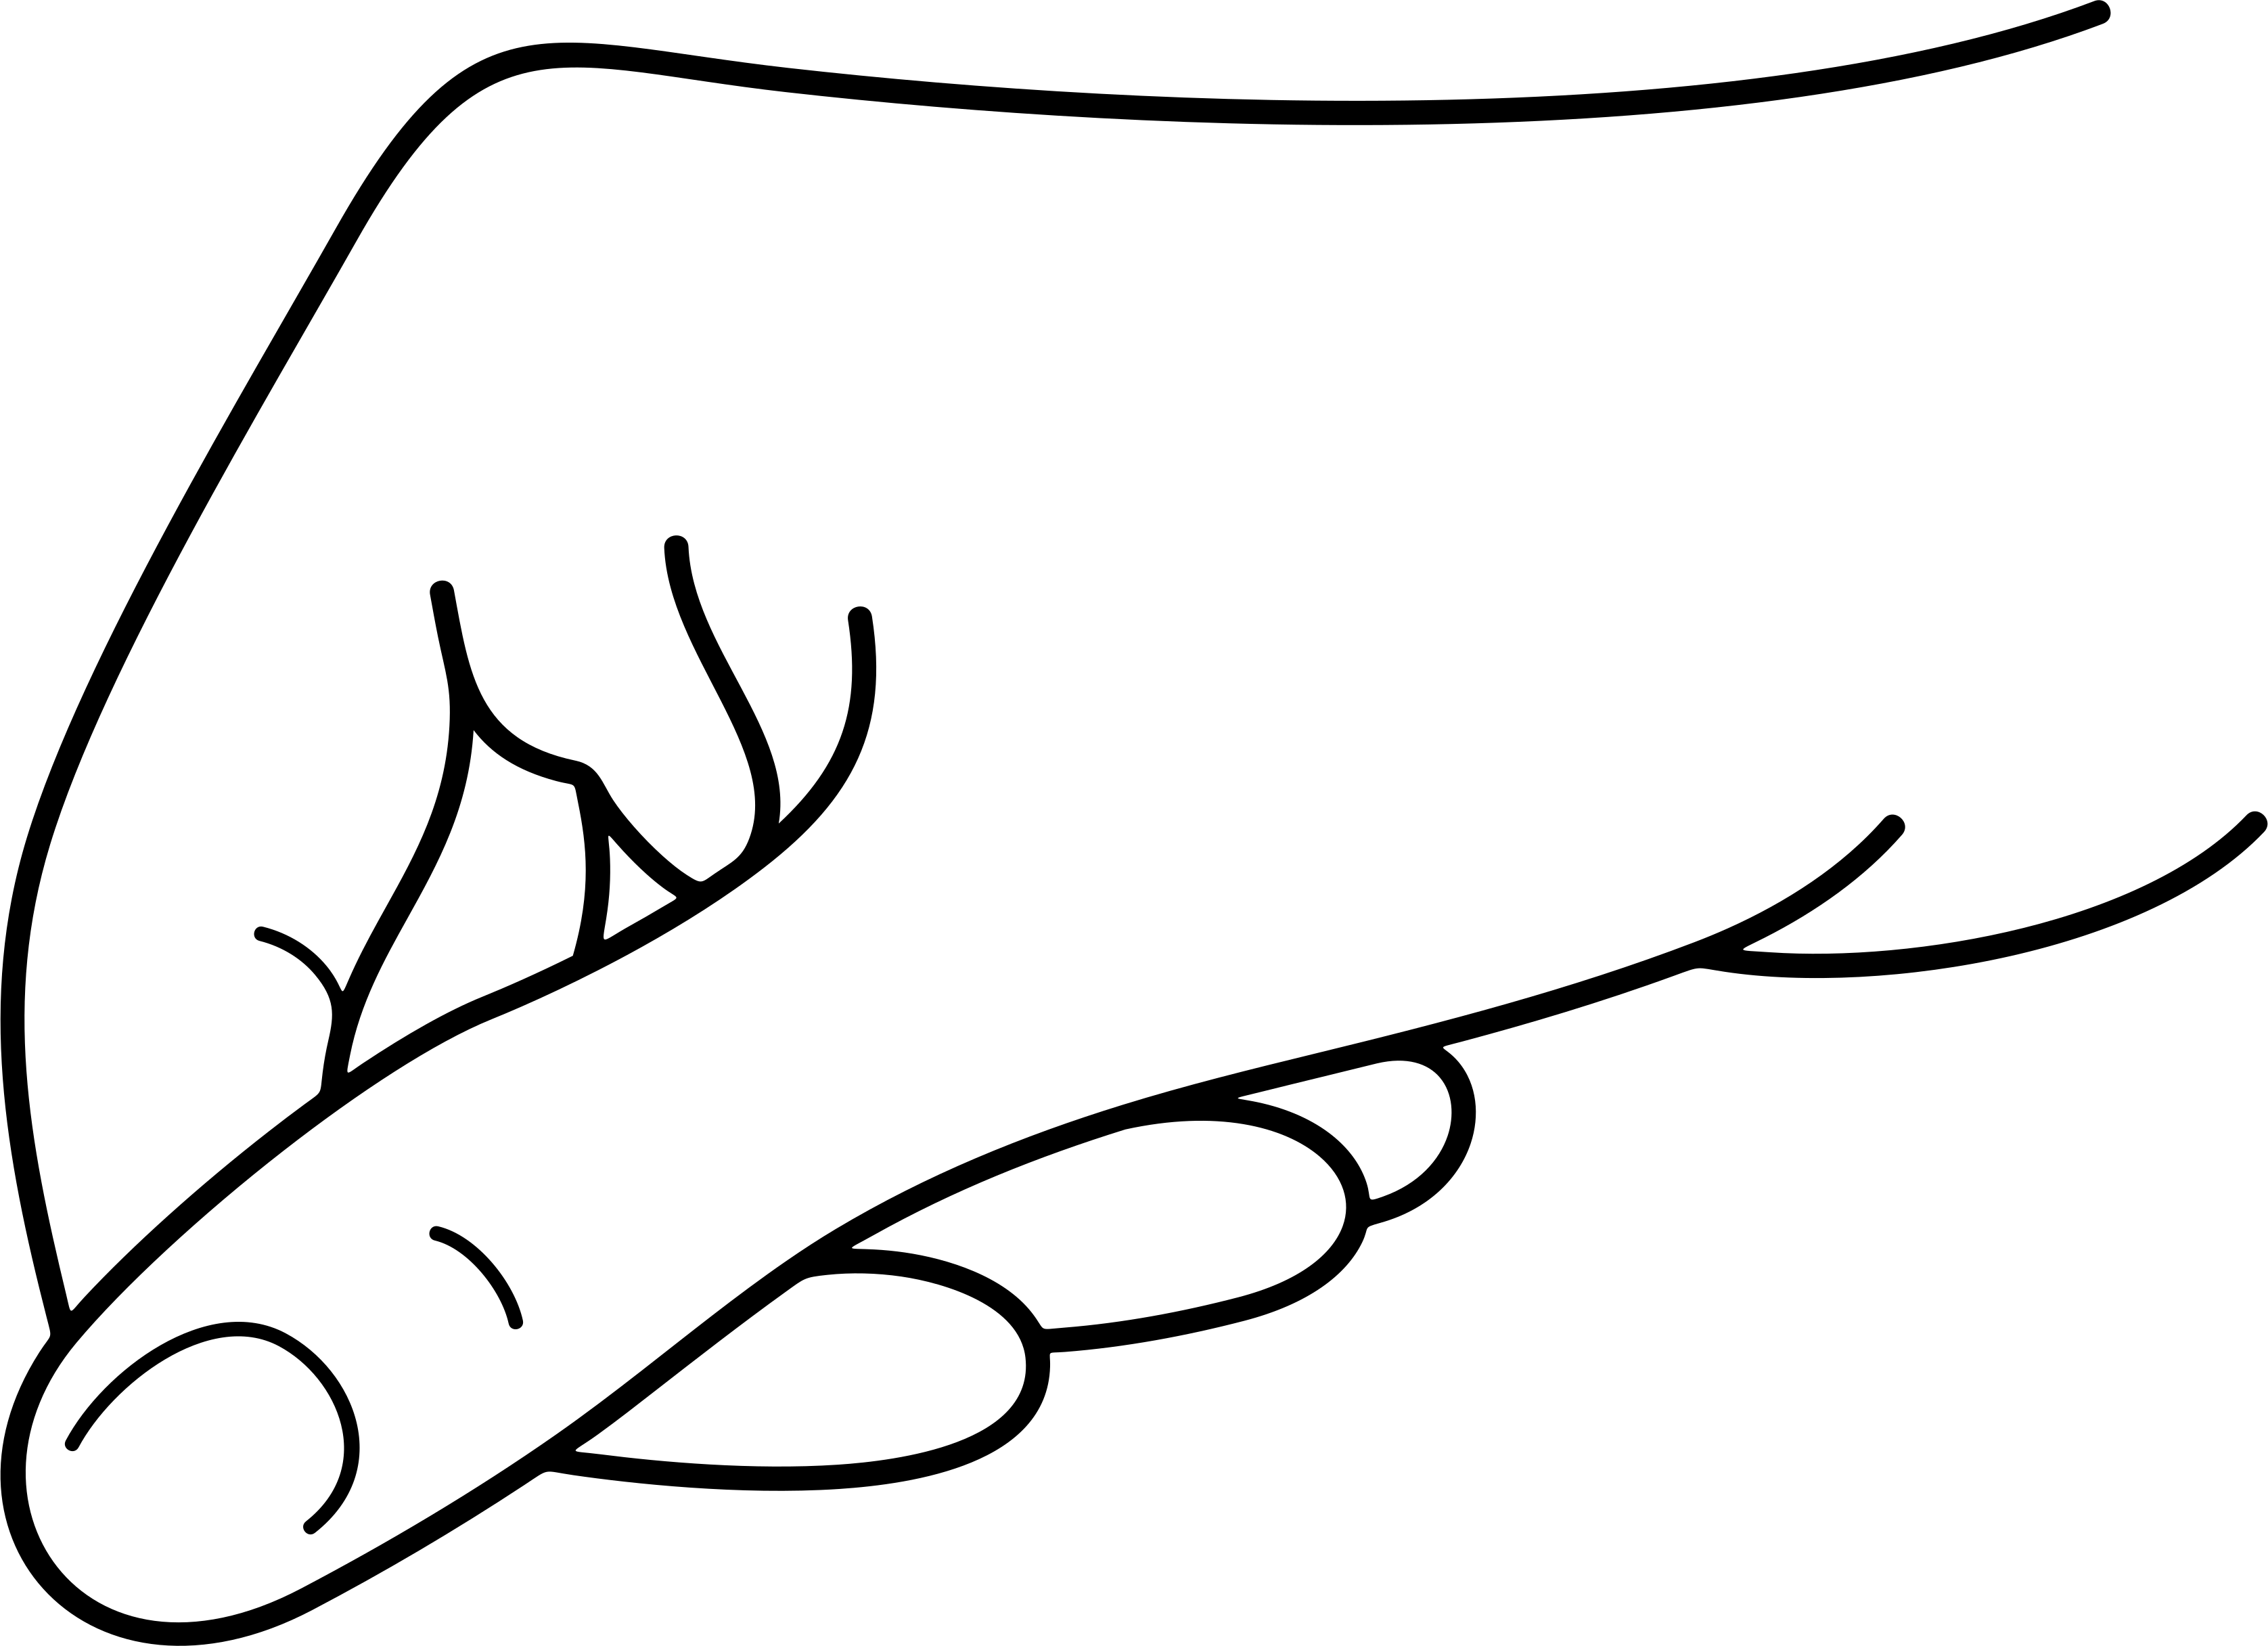
\includegraphics[width=1cm]{clipart/grab}};
	}

\snshonslide{4-}{3}{1-}{\xcoord{6}{0.15}
	\draw [decorate,decoration={coil,aspect=0.3,segment length=.3 cm,amplitude=3mm}] (0,0.5)--(6.1,0.5);
	\draw (6.1,0.5)--+(.5,0);
	\draw (6.5,.75)node[right]{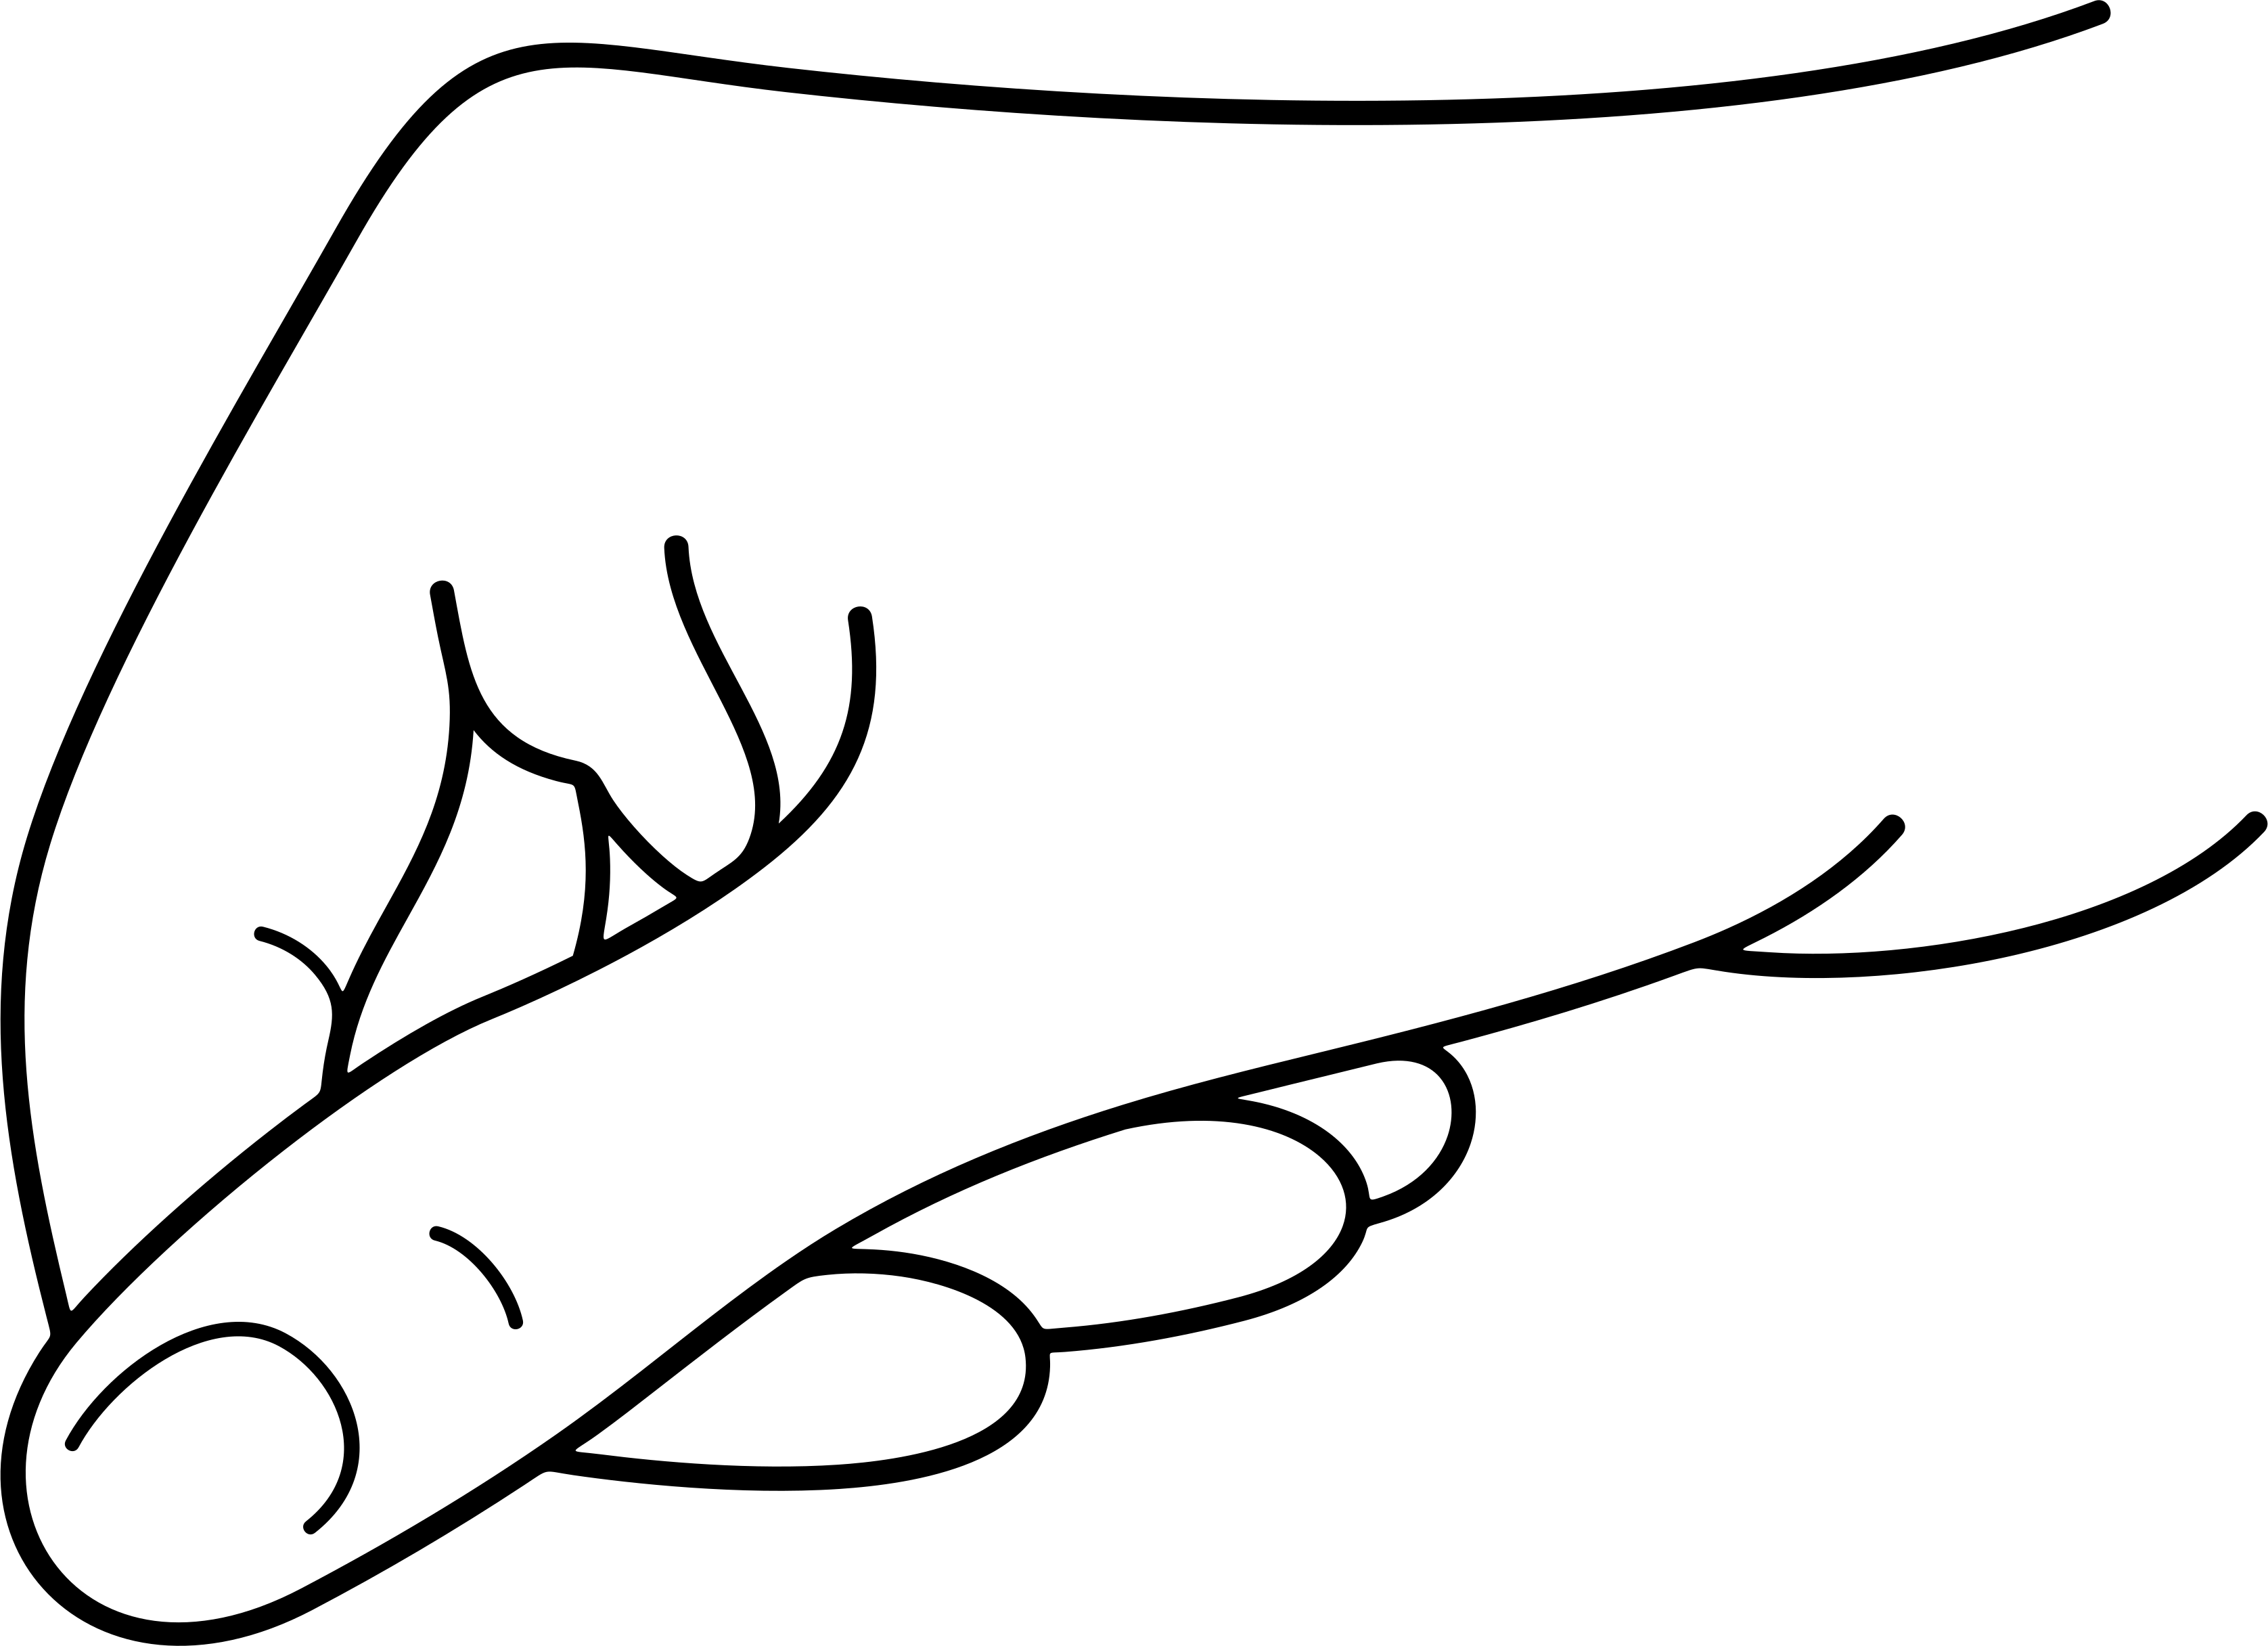
\includegraphics[width=1cm]{clipart/grab}};
	}
\end{tikzpicture}
\end{center}
\sonly<3>{


When the spring is stretched to 0.12 m, the force exerted is
\[k(0.12-0.1)=0.02k=12 N\]
So, $k = \frac{12 \text{ N}}{0.02\text{ m}}=600~~\frac{\text{N}}{\text{m}}=600~\frac{\text{kg}}{\text{s}^2}$.
}
\sonly<5->{
	The spring starts at 0.02 metres beyond its natural length, and ends 0.05 metres beyond its natural length. The work required is:
\begin{align*}
\int_{0.02}^{0.05}kx\ \dee x & = \int_{0.02}^{0.05}600x\ \dee x =\left[300x ^2\right]_{0.02}^{0.05}\\
&=300\left[0.05^2-0.02^2\right]=0.63~\frac{\text{kg m}^2}{\text{s}^2}=0.63~\text{J}
\end{align*}
	}

\unote{Example~\eref{text}{eg:WKspring}}
\end{frame}%----------------------------------------------------------------------------------------

%----------------------------------------------------------------------------------------
